\section { Design }

\subsection{Multithreading}
In order to maximise ease-of use, the software should have a graphical user environment (GUI) so that the current audio being played can be easily visualised (in-line with objective 2). The program will use a multithreaded model, with a separate "audio thread" and "GUI thread", allowing the two to run concurrently without blocking each other's processing.

\begin{figure}[h]
	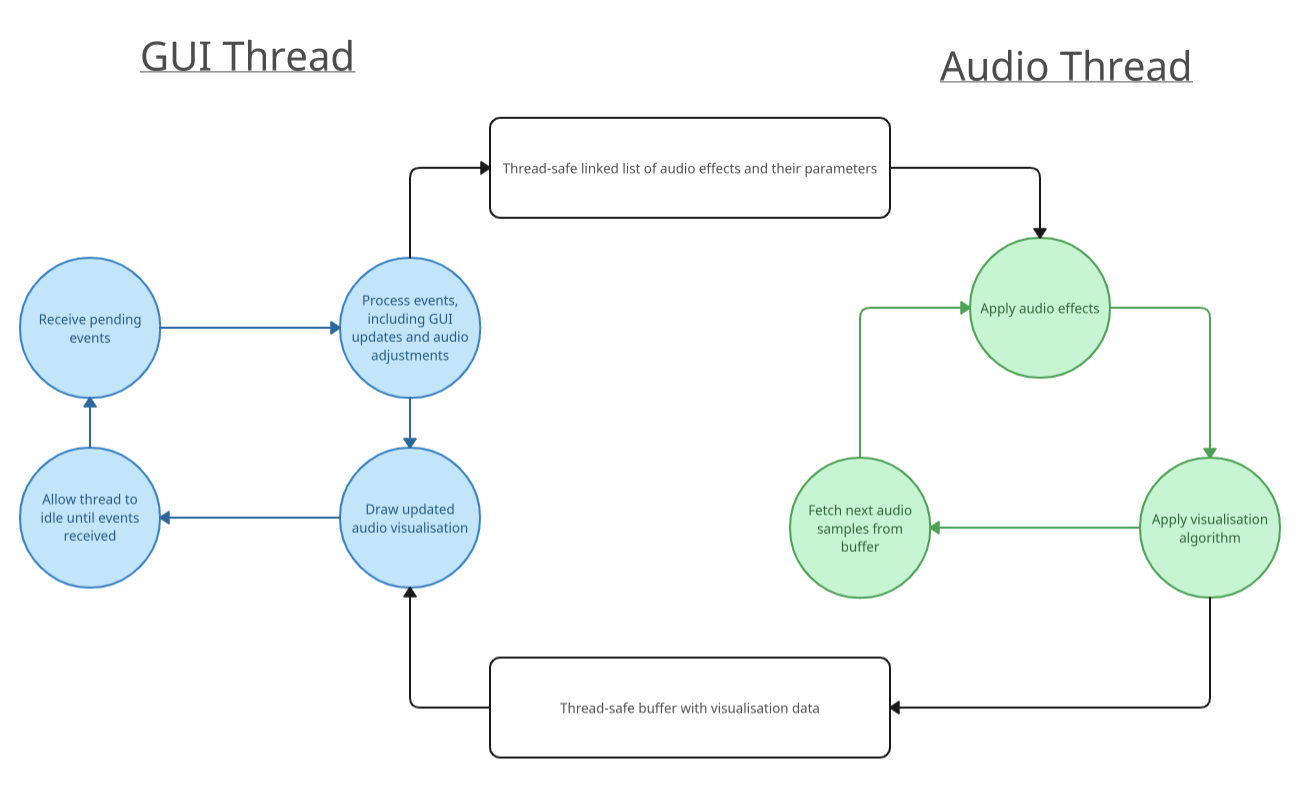
\includegraphics[width=17cm]{./threading.png}
	\caption{Inter-thread diagram - see below for justification for thread-safe data structures}
\end{figure}

\paragraph{}
Typically, GUI programs are written using an event-based paradigm that minimises CPU idle-time. The consequence of this is that, for most of the time, the GUI thread is suspended, awoken only when events from the user (such as mouse clicks or resizing the window) "wake it up". This is desirable in order to minimise system resources used, as more CPU-time will be available for the audio processing requirements, helping to reach the real-time requirements of objective 6. However, this presents a unique challenge. With a single-threaded model:
\begin{itemize}
	\item If the event-based model is followed, the GUI thread is only active when there are pending GUI events to be processed, meaning audio processing can only occur sporadically (resulting in "non-constant" audio)
	\item If instead the GUI thread is constantly active processing audio it will never reach a point where it can process pending events, meaning the program will hang and refuse to process inputs.
\end{itemize}

Hence it is desirable to split the program into two distinct threads. The audio thread can play the audio and perform all necessary processing tasks, whilst the GUI thread can relay input parameters and commands to the audio thread (such as "switch song", "apply effect", etc.).

\paragraph{}
To avoid race conditions\footnote{
	 Race conditions occur when one thread tries to read data whilst the other writes to it. If, for example, the GUI thread removed an audio effect from the audio effect list (see above) and freed it from memory whilst the audio thread was applying that same effect, the audio thread would suddenly be reading from invalid memory, likely resulting in a crash or undefined behaviour.
}, the data that is read by both threads should be thread-safe - only one thread should be able to access the data at a time. This can be achieved by using mutexes\footnote{
	A mutex is an object that prevents multiple threads from accessing data at the same time. It can be thought of as a lock, which can only be unlocked for one thread at a time. They are preferable to spinlocks as they do not require the CPU to waste cycles waiting for the data to be "unlocked", as instead the thread can suspend itself until the mutex becomes available.
}.

\subsubsection{Audio Effects Data Structure}
\paragraph{Picking a data structure} The user will likely want to adjust the order of audio effects at will, and as the same time, it must be very fast to insert and  remove audio effects so as to minimise the time spent not processing audio (even a very short pause may result in "crackles" on weaker hardware). To solve this problem, the audio effects can be stored in a linked list, as unlike std::vectors (dynamic C++ arrays) they prove fast insertion, deletion and swapping irrespective of the number of elements stored.

\paragraph{Making it thread-safe}
To satisfy the requirements of multithreading (see above), I will write my own custom "atomic linked list", backed by a mutex\footnote{
	See above footnote on mutexes
}, which will function just like a normal linked list but maintain thread-safety in all its operations.


\pagebreak

\subsection{Audio Data and Playback}

\subsubsection{Audio Data}
The program will have to load a variety of  user-supplied data in order to operate:
\begin{itemize}
	\item As described in objective 1, the user must be able to load a collection of audio files known as  a "playlist", which will contain the paths of one or more audio files on the system.
	\item Each audio file will consist of a number of audio samples, which will need to be loaded into memory when needed, then freed when not in use.
	\item Audio files also contain other crucial information, such as the audio frequency (e.g. 44,000 Hz), the number of channels (usually mono (1) or stereo (2)), and the number of samples (the "length").
	\item Thus to keep track of the audio files loaded into memory, each audio file will need to store its raw audio samples, its frequency, the number of channels, and the number of samples.
\end{itemize}

\subsubsection{ Audio Data UML }
\begin{figure}[H]
	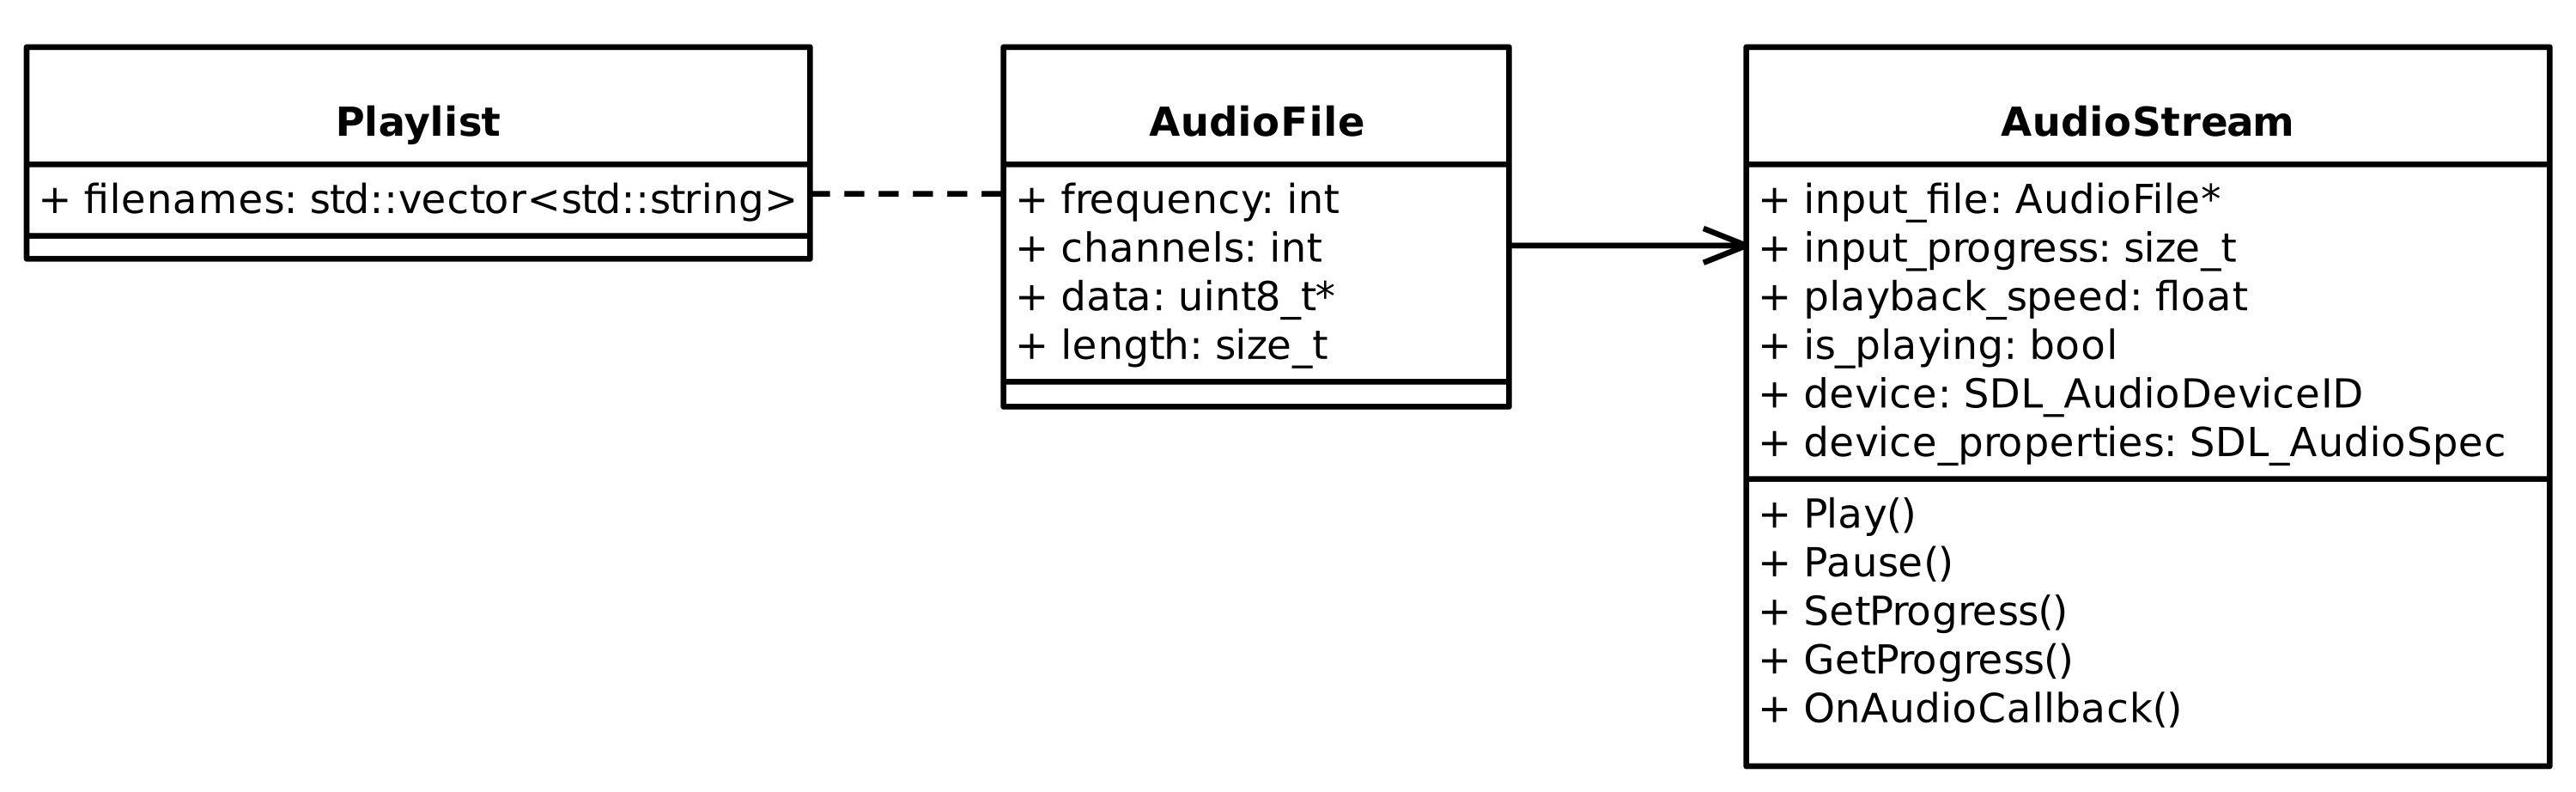
\includegraphics[width=14cm]{./audio io uml.png}
	\caption{UML for Audio Data and IO - separate getter and setter exists for AudioStream progress as the caller will express progress as percentage (e.g. 50\% played) so that it is independent of file size. The playlist contains the filenames of all audio files on disk, and an AudioFile instance is created, when needed, by loading the audio file from disk using this filename. }
\end{figure}

\subsubsection{The Need for Streaming}
It may be tempting to load and unload all audio data in a hierarchal  fashion as such:
\begin{enumerate}
	\item An attempt is made in the code to load a playlist.
	\item To do this, the playlist will be read from disk and all the audio file paths contained within will be loaded into memory.
	\item Each audio file path will be verified to check it is valid exists on the system.
	\item If the playlist is valid, each audio file will then be loaded using the paths provided.
	\item Thus the loading of a playlist will involve loading all audio files referenced within.
	\item At the end of the program, when the playlist is no longer needed, all the playlist's audio files will be freed from memory, followed by the playlist itself.
\end{enumerate}

However, this is not a practical approach due to memory usage constraints. If a user attempted to load a playlist consisting of 200 songs, each 5 MB each, this would consume roughly 1000 MB of memory for the entire duration of the program, even though only 1 audio file can be played at once (and hence only one needs to be in memory at any one time). This conflicts with objective 6 ("the system must run in real-time on an average school computer") as many computers may not have large amounts of free memory, particularly if other programs are running, which may lead to an out-of-memory crash.

\paragraph{}
Instead, I have decided to "stream" audio files as they are played, so that only the audio file currently needed is resident in memory. This can be modelled as followed:
\begin{enumerate}
	\item An attempt is made in the code to load a playlist.
	\item To do this, the playlist will be read from disk and all the audio file paths contained within will be loaded into memory.
	\item Each audio file path will be verified to check it is valid exists on the system. If the playlist is valid, the execution of the program will continue.
	\item Each time the next audio file is to be played from the playlist, the program will dynamically load it from disk (using the path from the playlist) and store it in memory.
	\item When the next audio file is chosen, it is loaded as described above. Crucially however, the previous audio file is first unloaded from memory, as it is no longer needed.
	\item At the end of the program, the currently playing audio file and playlist are both freed.
\end{enumerate}

\paragraph{}
In this way, the issue of large playlists resulting in extremely large memory consumption will be avoided, as only one audio file will be loaded at once.

\subsubsection{Audio Playback}
The playback of audio itself presents many challenges. In order to make the code as modular and decoupled as possible, I will abstract away the low-level creation of audio devices, pausing, un-pausing, etc. into an "AudioStream" class. One will simply create an "AudioStream", supply it with data, and the class will manage the various complexities of multithreading and feed the audio buffer with data at the appropriate times.

\paragraph{}
In order to maximise portability of the code,  and hence make it as cross-platform as possible in order to maximise the program's audience, I have decided to use a library called "SDL2" to handle audio playback, as it abstracts away the native APIs one would have to otherwise use. In this way, separate audio code does not have to be written for Windows, Linux, etc.

\paragraph{}
The code that plays audio on the system will run on a separate thread (see multithreading section). This audio thread is invoked at regular intervals by the operating system by way of a "callback" function. When this happens, it is the program's responsibility to supply the operating system with the next buffer of audio. This is summarised below:

\begin{enumerate}
	\item An "AudioStream" is created and supplied with the raw audio samples from the audio file, as well as pointers to the atomic linked list of audio effects and to the visualisation data buffer.
	\item The AudioStream uses SDL2 to invoke audio playback at regular intervals on a separate thread (the "audio thread") using a callback
	\item Every time the callback is called, the AudioStream will fetch the next section of upcoming audio that it has been supplied with.
	\item If playback speed has been modified, the audio must be "stretched" or "squashed down" (discussed in more detail below)
	\item Each audio effect will then be applied (using the audio effects atomic linked list).
	\item The audio visualisation module will then be invoked on the audio just processed, and its output written to the visualisation data buffer.
	\item Now that all work is done for the current section of audio, the processed audio will be copied to the callback's audio buffer and the audio thread will suspend itself.
	\item When the next section of audio is due, the callback will be re-invoked.
\end{enumerate}

\subsubsection { Audio Playback Flowchart }
\begin{figure}[H]
	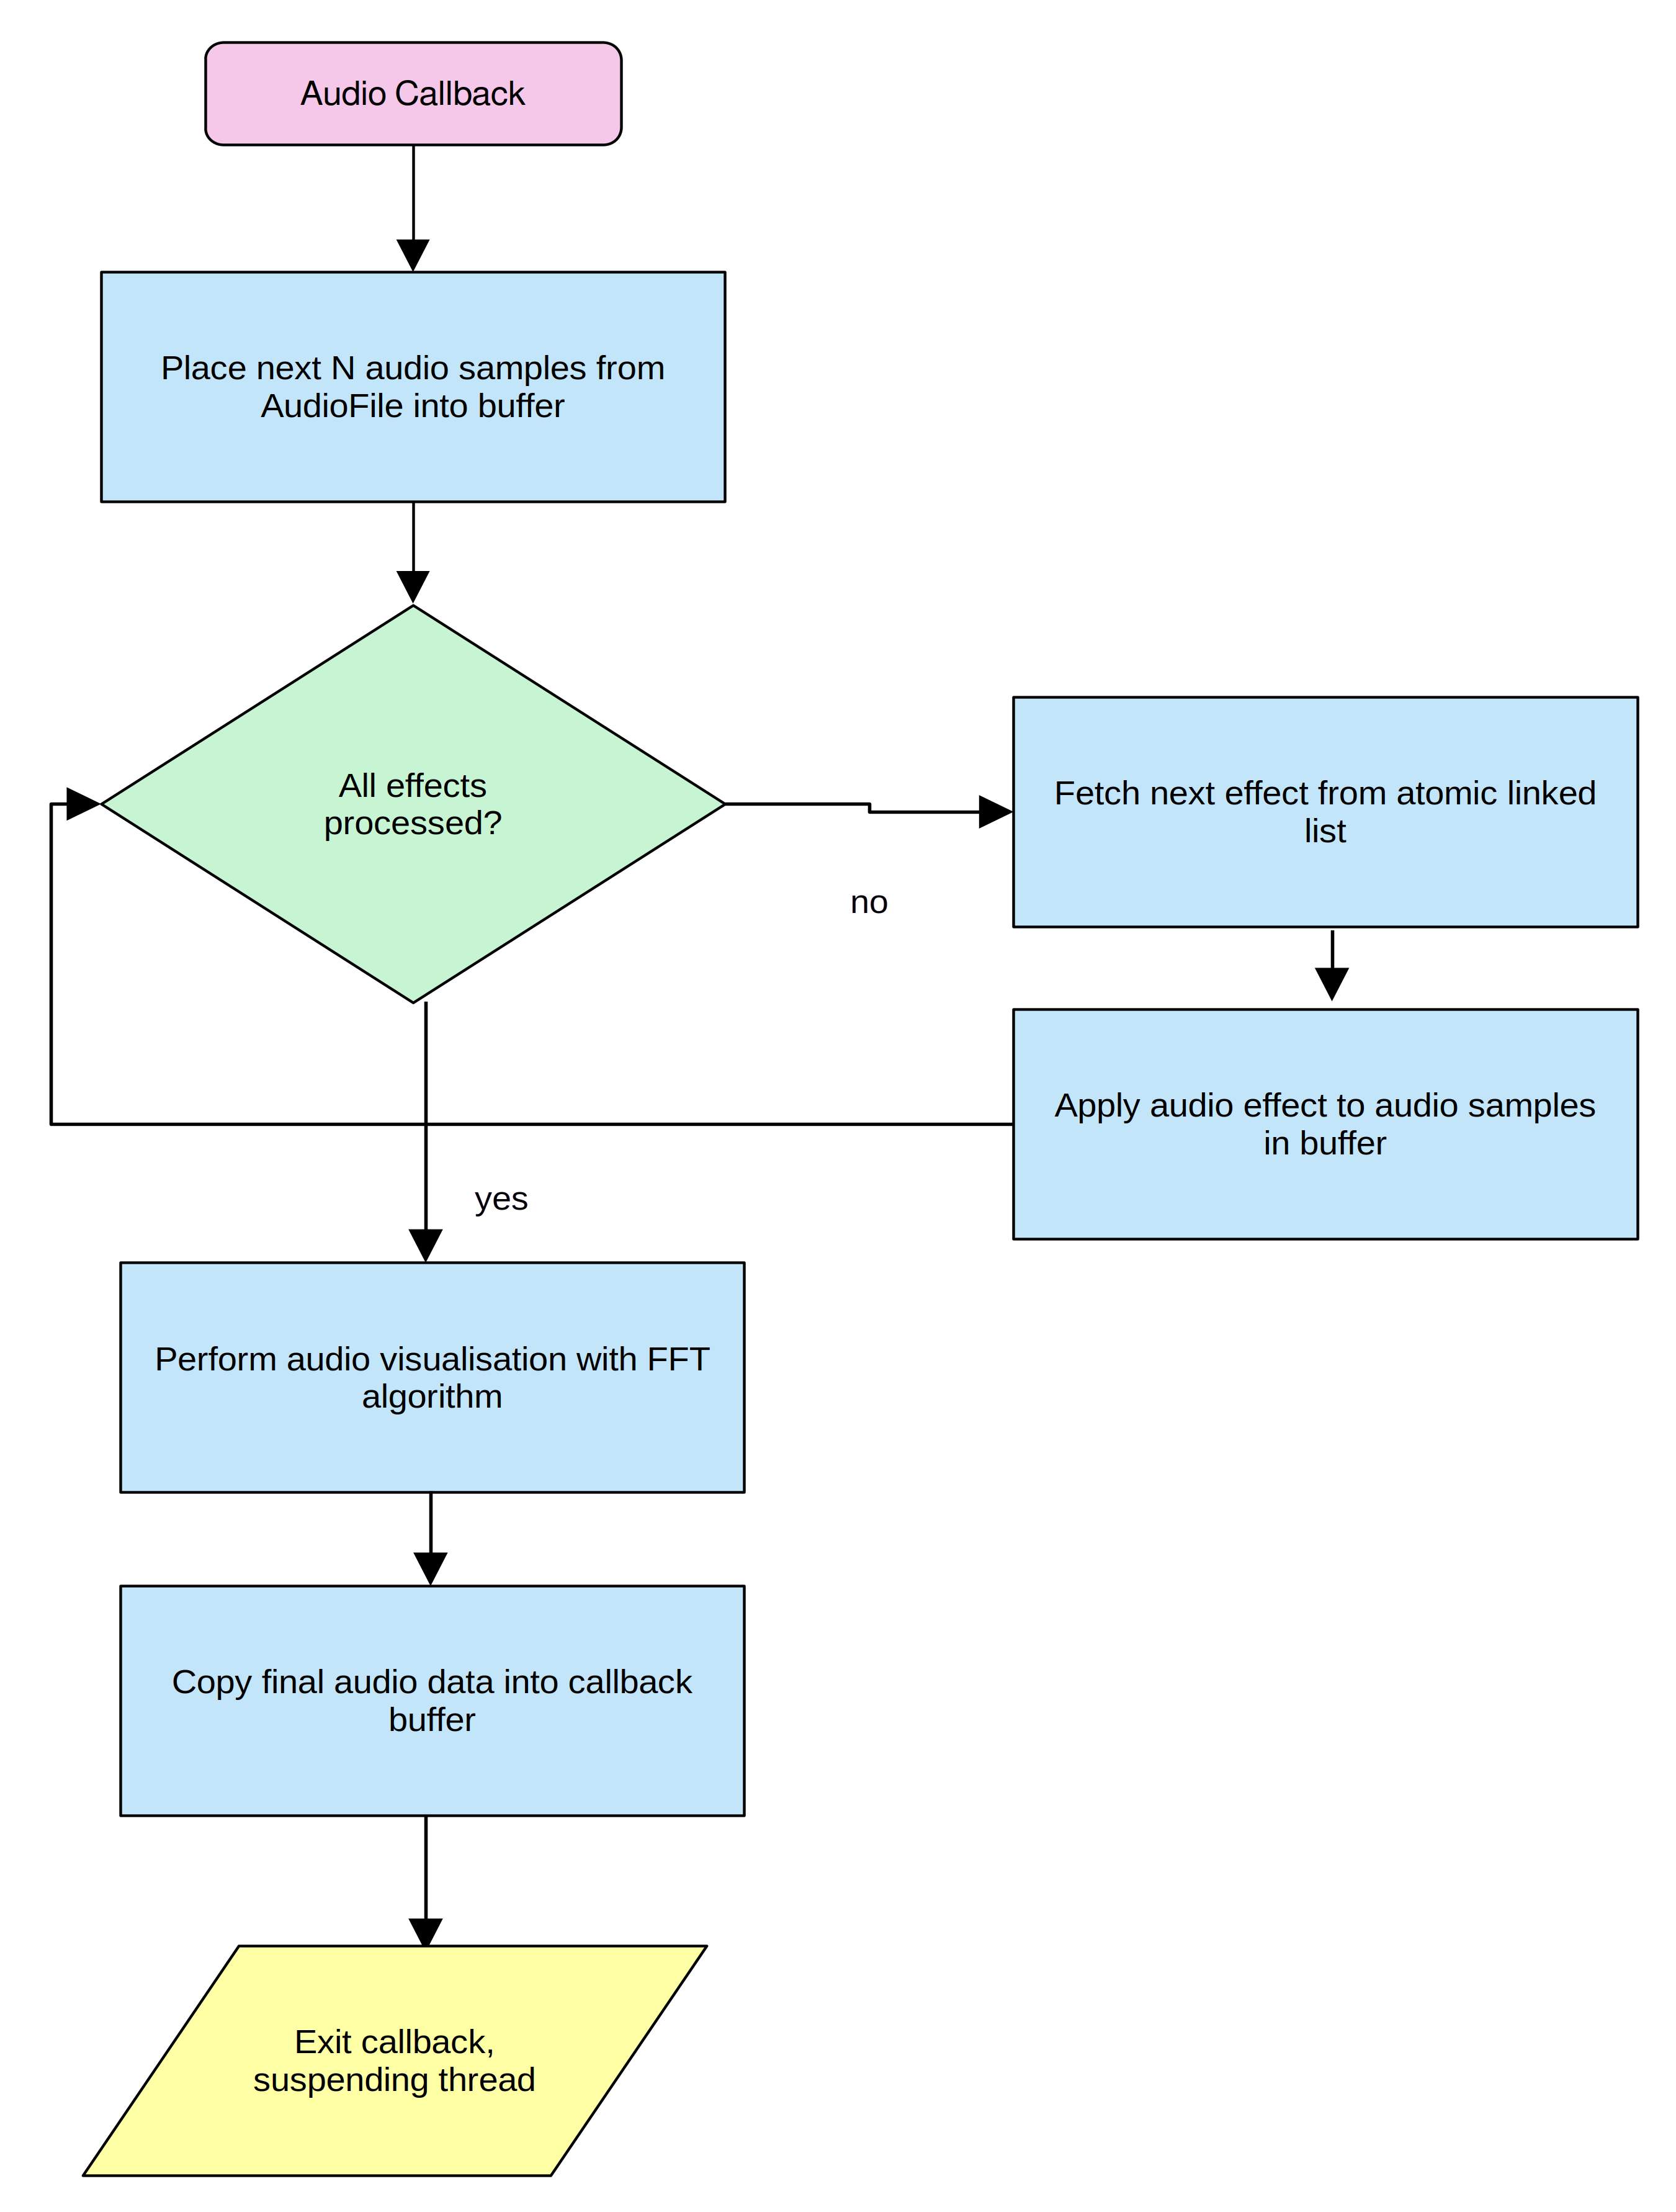
\includegraphics[width=14cm]{./audio io flowchart.png}
	\caption{Flowchart for AudioStream's SDL audio device callback}
\end{figure}

\subsubsection{Adjusting Audio Playback Speed}
\paragraph{}
As discussed above, if the audio playback speed has been modified, then there is a need to "resample" the audio. Imagine, for example, we wish to play music at twice the speed. In the audio callback subroutine, we have therefore fetched twice as many audio samples, as we wish to fit twice as much audio into a single period of time. However, the audio output buffer only has a fixed length, so we must "squash" the larger (normal speed) buffer into the smaller output buffer, which will double its speed. One can imagine the same process applies to slowing down audio, but instead we must "stretch" the audio instead by copying a smaller input buffer (as we have fetched less audio) into the larger output one.

\paragraph{}
To do this I have designed the following pseudo-code:
\begin{minted}{ada}
function ResampleBuffer(buffer: array of float) -> array of float:
	-- No need to re-sample if we're already at 1x speed
	if input_speed is 1.0:
		return buffer
	
	-- Allocate output buffer
	target_size := round(size of buffer / input_speed)
	output := new empty array of float with size target_size
	
	-- Copy input buffer to output in "input_speed"-sized steps
	-- e.g. if input speed is 2x, skip every 2nd audio sample
	-- e.g. if input speed is 0.5x, insert every audio sample twice
	curret_index := 0.0
	while curret_index < size of buffer:
		append buffer[round(curret_index)] to output
		curret_index += input_speed
	
	return output	
\end{minted}


\pagebreak

\subsection{Audio Effects Architecture}
The full list of audio effects detailed in the analysis section is as follows:
\begin{itemize}
	\item Equaliser (frequency modification) - selectively modifying frequencies such as by altering the bass
	\item Echo - making audio sound like it's recorded in a large room
	\item Volume adjustment - modifying the amplitude of the audio
	\item Noise - adding subtle imperfections to the audio
\end{itemize}

\subsubsection{Unique Audio Effect Traits}
Each audio effect will need its own properties, and potentially its own mutable state (for example, the echo effect needs to "remember" the previous audio samples so it can repeat them later). Below is a summary of the requirements, properties and state of each audio effect.

{
\renewcommand{\arraystretch}{1.5}
\begin{table}[h!]
	\begin{center}
		\begin{tabularx}{1.0 \textwidth} {
				| >{\raggedright\arraybackslash}X
				| >{\raggedright\arraybackslash}X
				| >{\raggedright\arraybackslash}X
				| >{\raggedright\arraybackslash}X  |
			}
			\hline
			Effects & Requirements & Properties & State \\

			\hline
			Equaliser & Allow the user to alter the volume of a selected frequency range. Multiple equaliser effects can be applied successively to cover multiple ranges.  & Lower frequency \newline  Upper frequency \newline Multiplier  & None \\

			\hline
			Echo & Produce an echo effect where audio sounds like it's getting reflected in a large room & Fall-off (how quickly echoes fade) \newline Delay samples (how many samples must pass before a sample is echoed) & Previous audio samples buffer \\

			\hline
			Volume & Adjust the volume / amplitude of incoming audio & Volume multiplier & None \\

			\hline
			Noise & Add subtle imperfections to the audio & Intensity (the volume of the noise) & None\\

			\hline
		\end{tabularx}
	\end{center}
\end{table}
}

\pagebreak
\subsubsection{Common Audio Effect Traits}
Immediately it is obvious that all audio effects will share many common features. Each effect shall:
\begin{itemize}
	\item Take a number of audio samples as input
	\item Have a number of configurable options which need to be exposed to the GUI front-end
	\item Perform processing on all audio samples at once
	\item Output its final processed audio
\end{itemize}

\paragraph{}
Given these requirements it is wise to use an object-orientated inheritance approach where effect subclass inherits from a common parent, which provides common functionality (such as the storage and exposing of configuration options), as well as providing a common interface that other parts of the code can use. In order to abstract away the details of interacting with an audio effect, two new classes will also be needed.

\subparagraph{Packet} A packet represents a chunk of audio awaiting processing by the effect. However, some effects require knowledge of both the previous audio samples and future audio samples\footnote{
	This is because performing Fourier transforms on isolated "chunks" of audio and then
	playing them back after modification will result in a periodic "clicking" sound at the boundary between chunks due to sudden changes in sound amplitude. This is because
	of the limited resolution of a Discrete Fourier Transform. To solve this, we must take
	into account both the sound packet that comes after, and the one that comes before.
}. Thus, each packet will consist of 3 audio buffers - one for the previous, current and next buffer of audio samples. A packet will also contain the frequency of the incoming audio as this is required for the FFT maths.

\subparagraph{Property} Each audio effect has a number of configurable properties. To aid in validation, each property will have a current,  minimum and maximum value.

\paragraph{}
Both these classes will be independent of the main audio effect parent class. The audio effect parent class will merely use these classes to represent the data provided and stored by it. This is an example of {\it composition}.

\subsubsection{Properties Data Structure}
Each audio effect will have a list of properties. When drawing a properties GUI, the front-end code will want an easy and convenient way of both getting a list of all available properties, along with their respective names. In a similar fashion, when setting the values of certain properties, it will be most convenient if properties can be accessed using their names.

\paragraph{}
I will use a hash-map as my data structure for this purpose. Hash-maps can be indexed by using the name of the property (e.g. "minimum frequency" as the key), simplifying the front-end code and avoiding the need for a separate "property name" variable. In addition, they provide very fast look-up with an O(1) time, which may be important if future effects have a large number of properties to avoid wasting CPU cycles iterating through properties (e.g. if stored in a list). Whilst hash-maps are expensive when it comes to adding and removing elements, each audio effect will only have a fixed number of properties that are added once at creation so this will not be an issue.

\paragraph{Polymorphism}
Some properties will be floating point values, whilst others will be integer values. If this project is continued further, I may wish to also add boolean values as well. To accommodate this, I will use polymorphism by creating a \textit{Property} base class, then \textit{FloatingPointProperty} and \textit{IntegerProperty}  children, which will share a common interface.

\subsubsection{UML Class Diagram}
After considering all the requirements of the multiple classes required, I have constructed a class diagram. However, a slight modification has been made to the typical UML structure: \textit{properties} of audio effects appear in the lower box in each class, in order to indicate that they are not attributes {\it per se}, but rather are elements in their parent's properties hashmap.

\begin{figure}[h]
	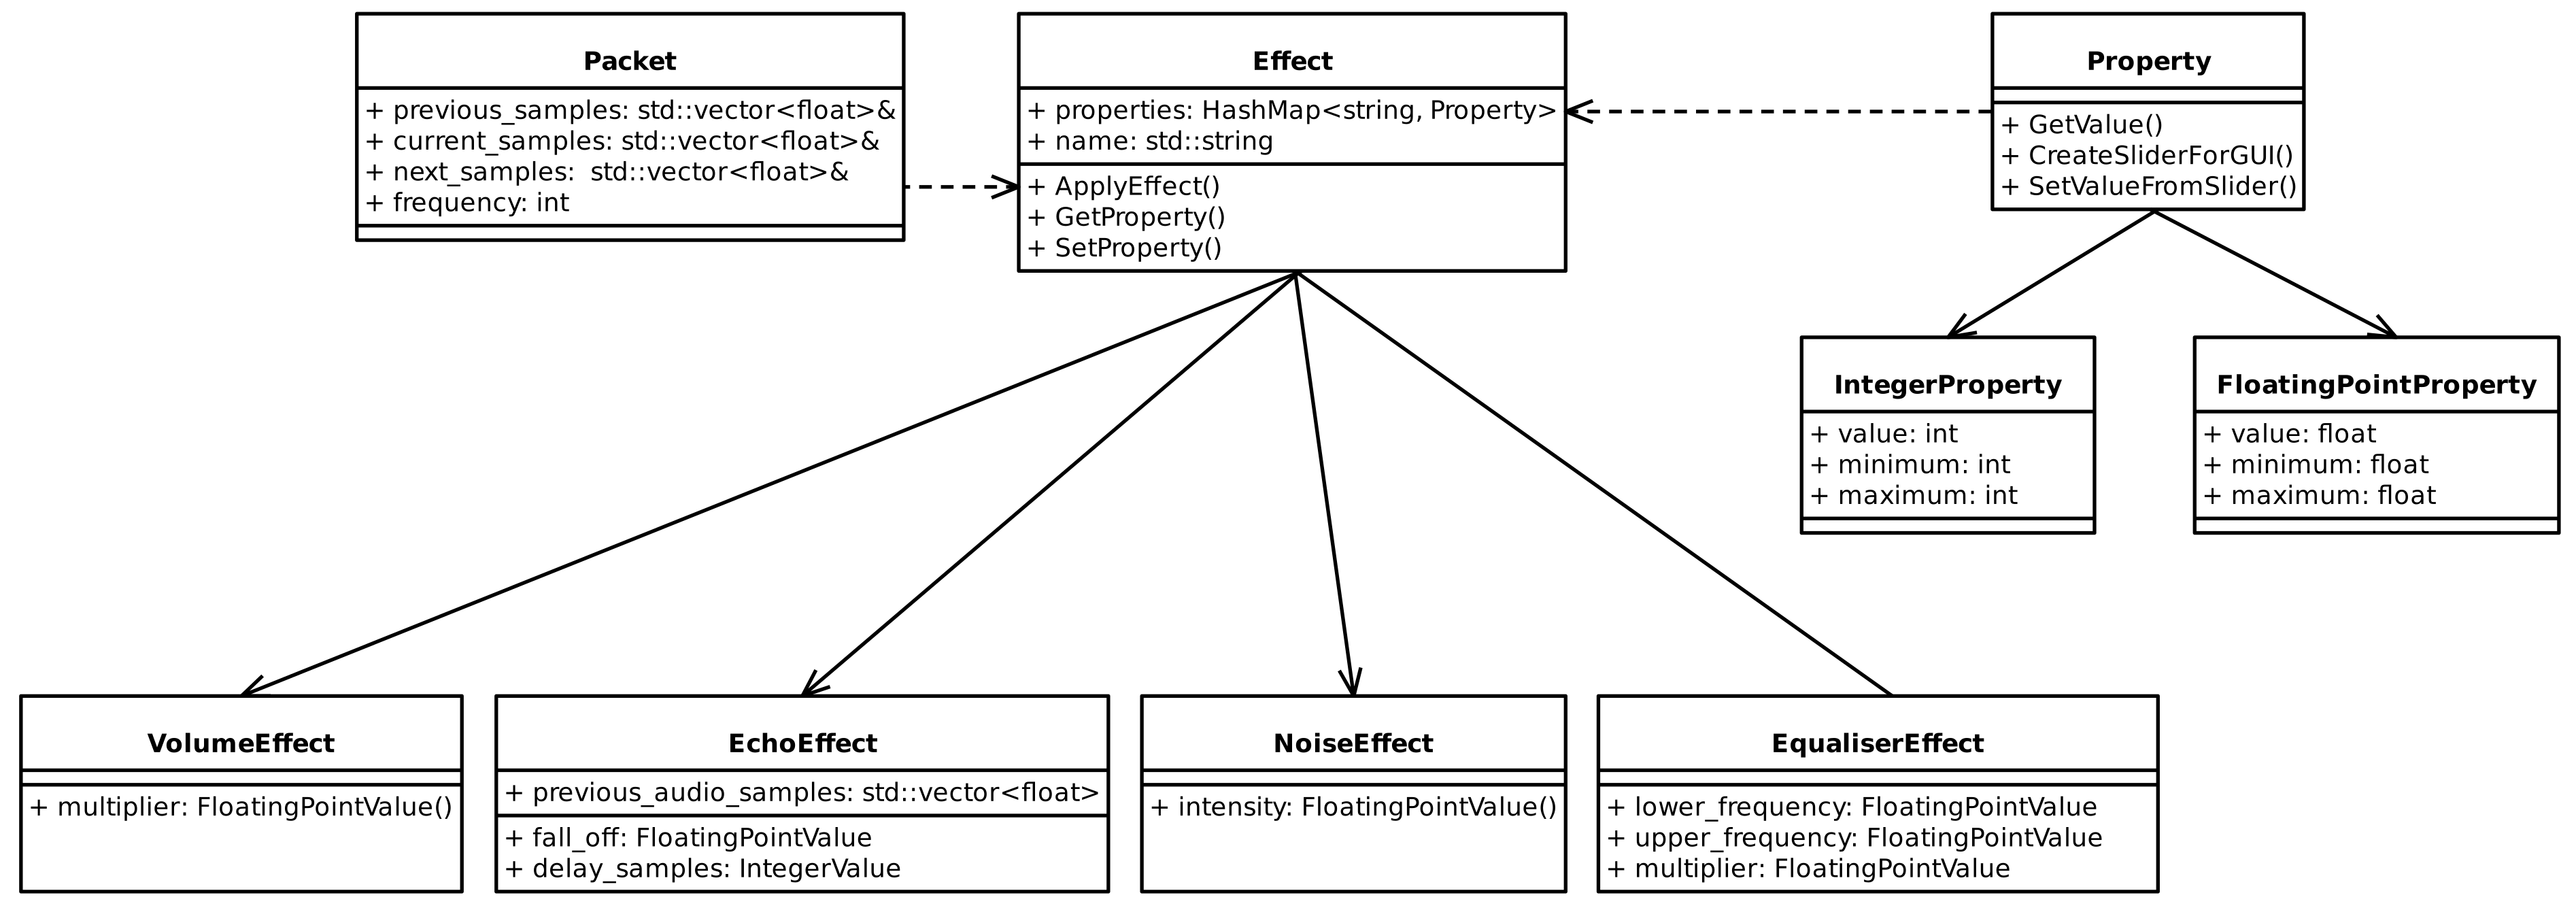
\includegraphics[width=\textwidth]{./effects class diagram new.png}
	\caption{UML class diagram containing attributes, operations and custom "properties"}
\end{figure}

\pagebreak

\subsection{High-Level Audio Effects Flowcharts}
\begin{figure}[H]
	\subsubsection{Equaliser}
	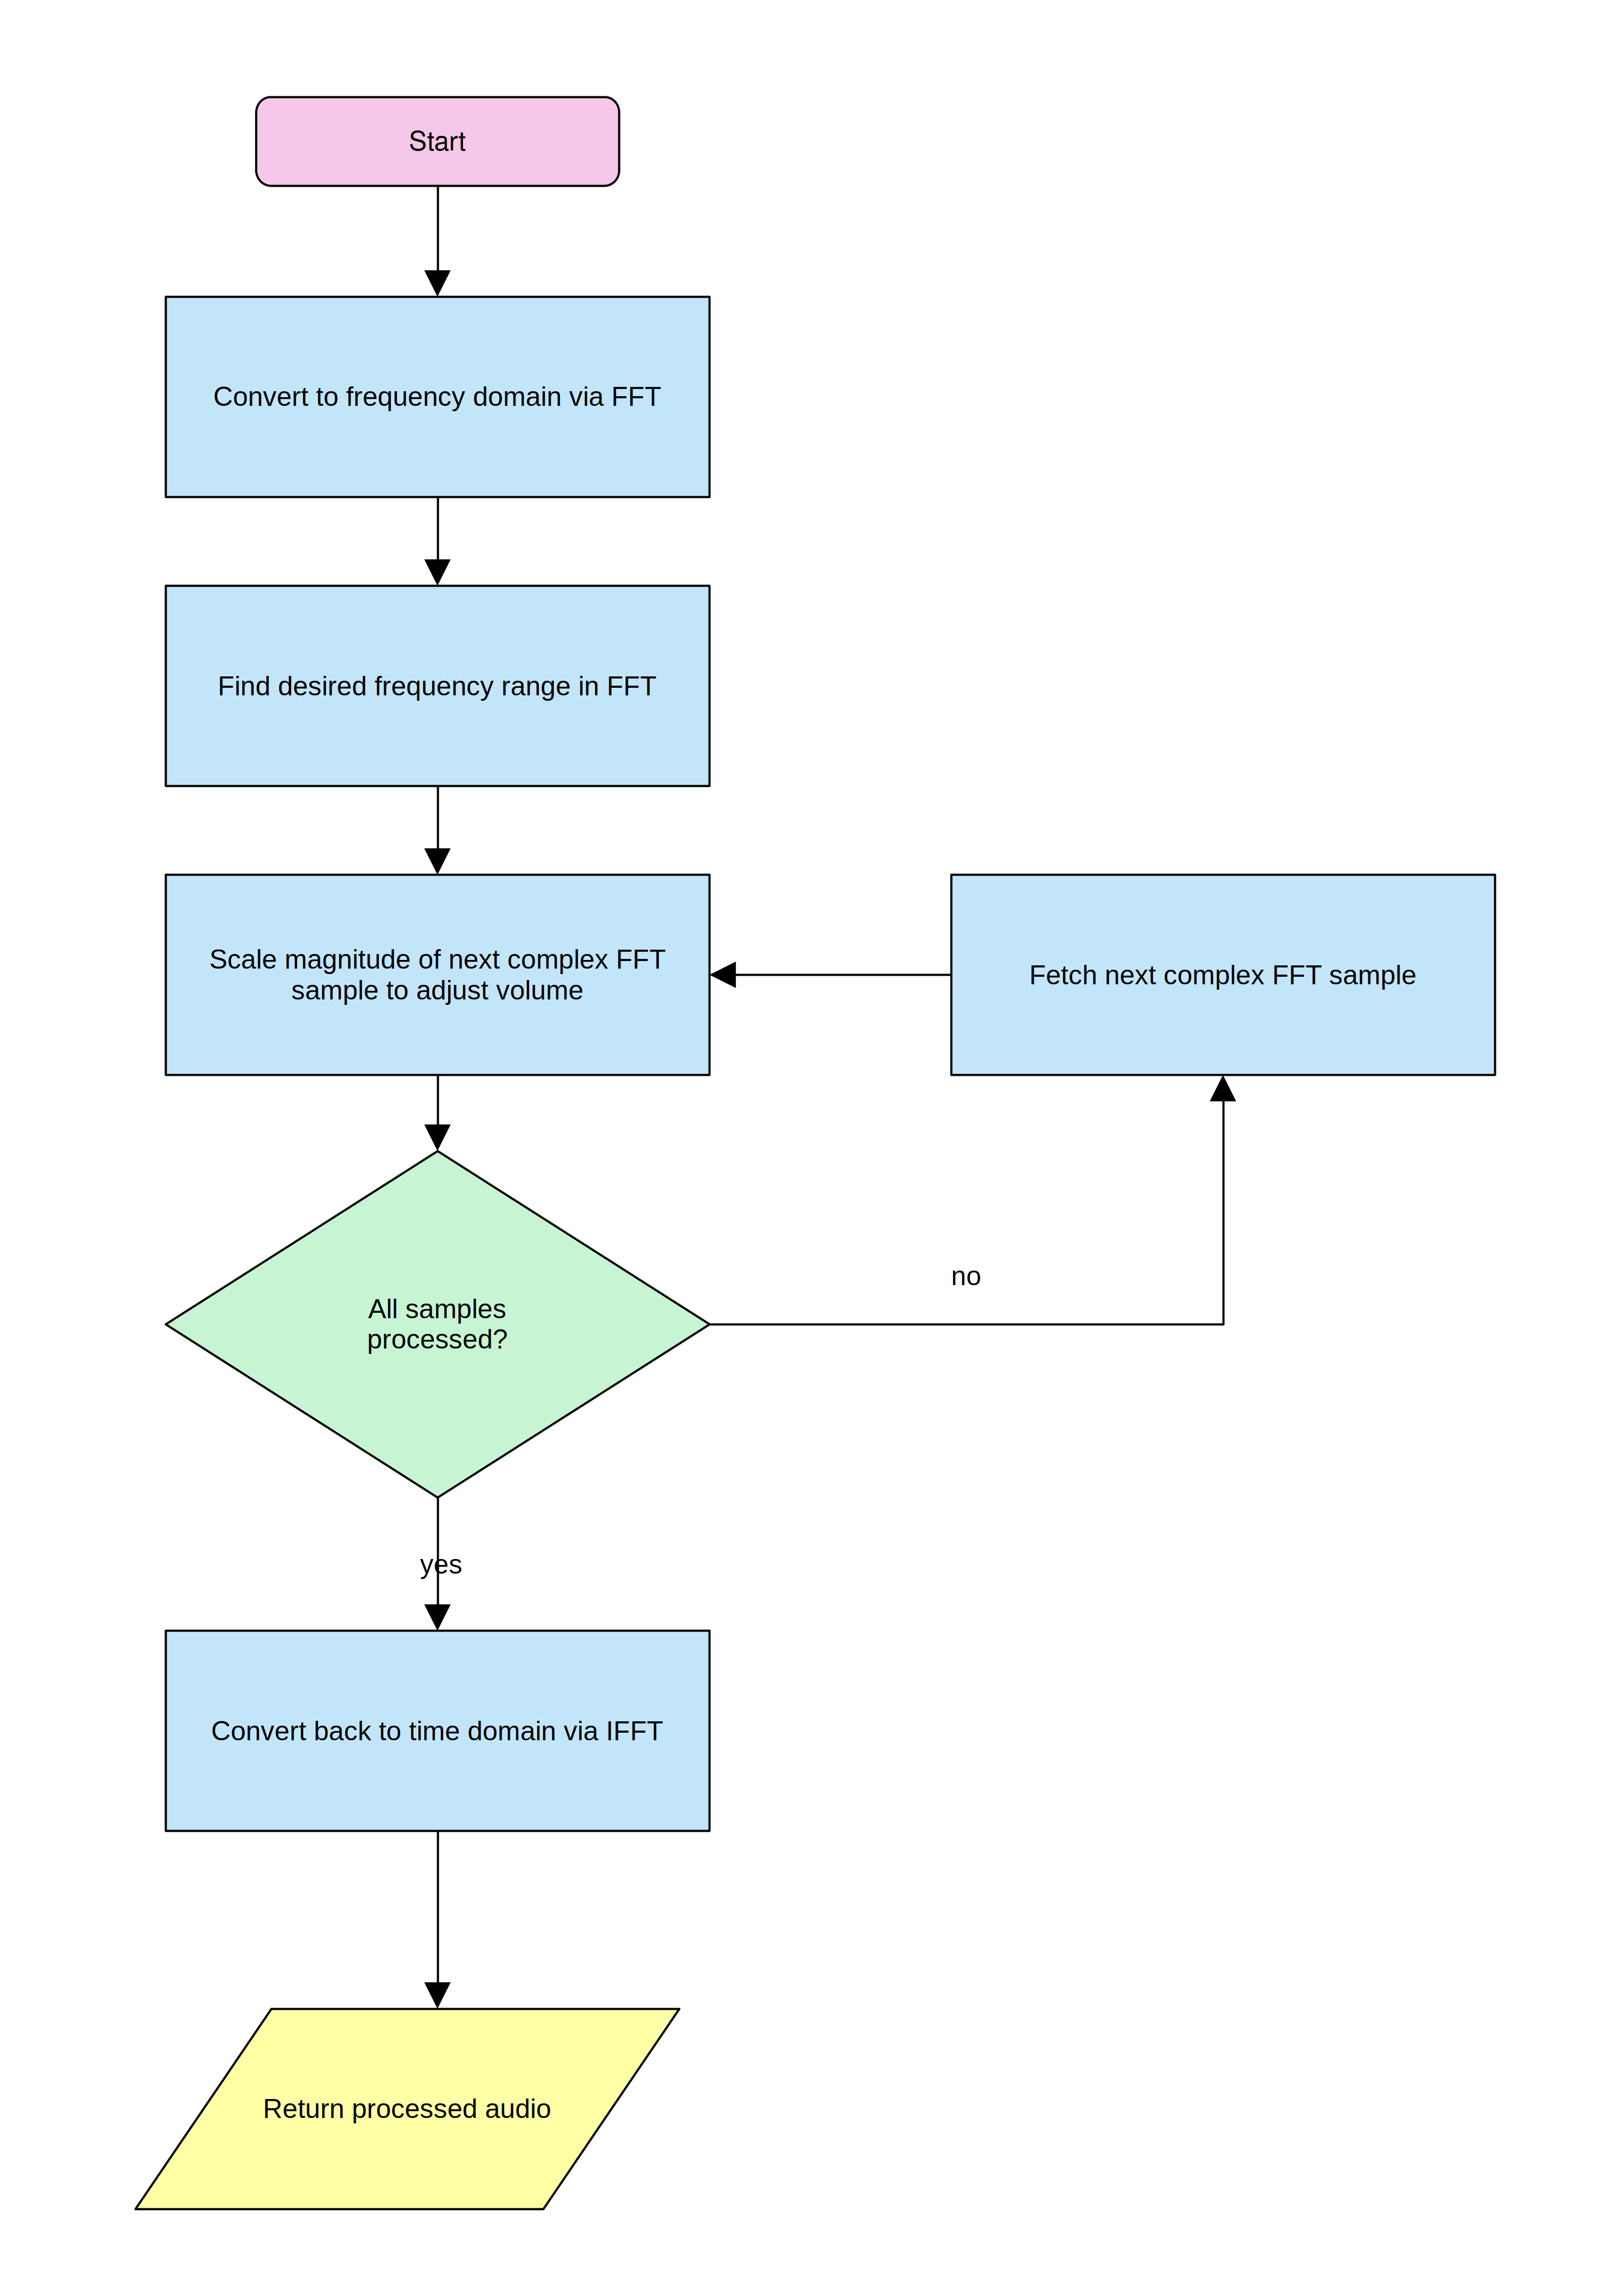
\includegraphics[width=14cm]{./equaliser flowchart.png}
	\caption{Flowchart for equaliser (frequency modification) audio effect}
\end{figure}

\begin{figure}[H]
	\subsubsection{Echo}
	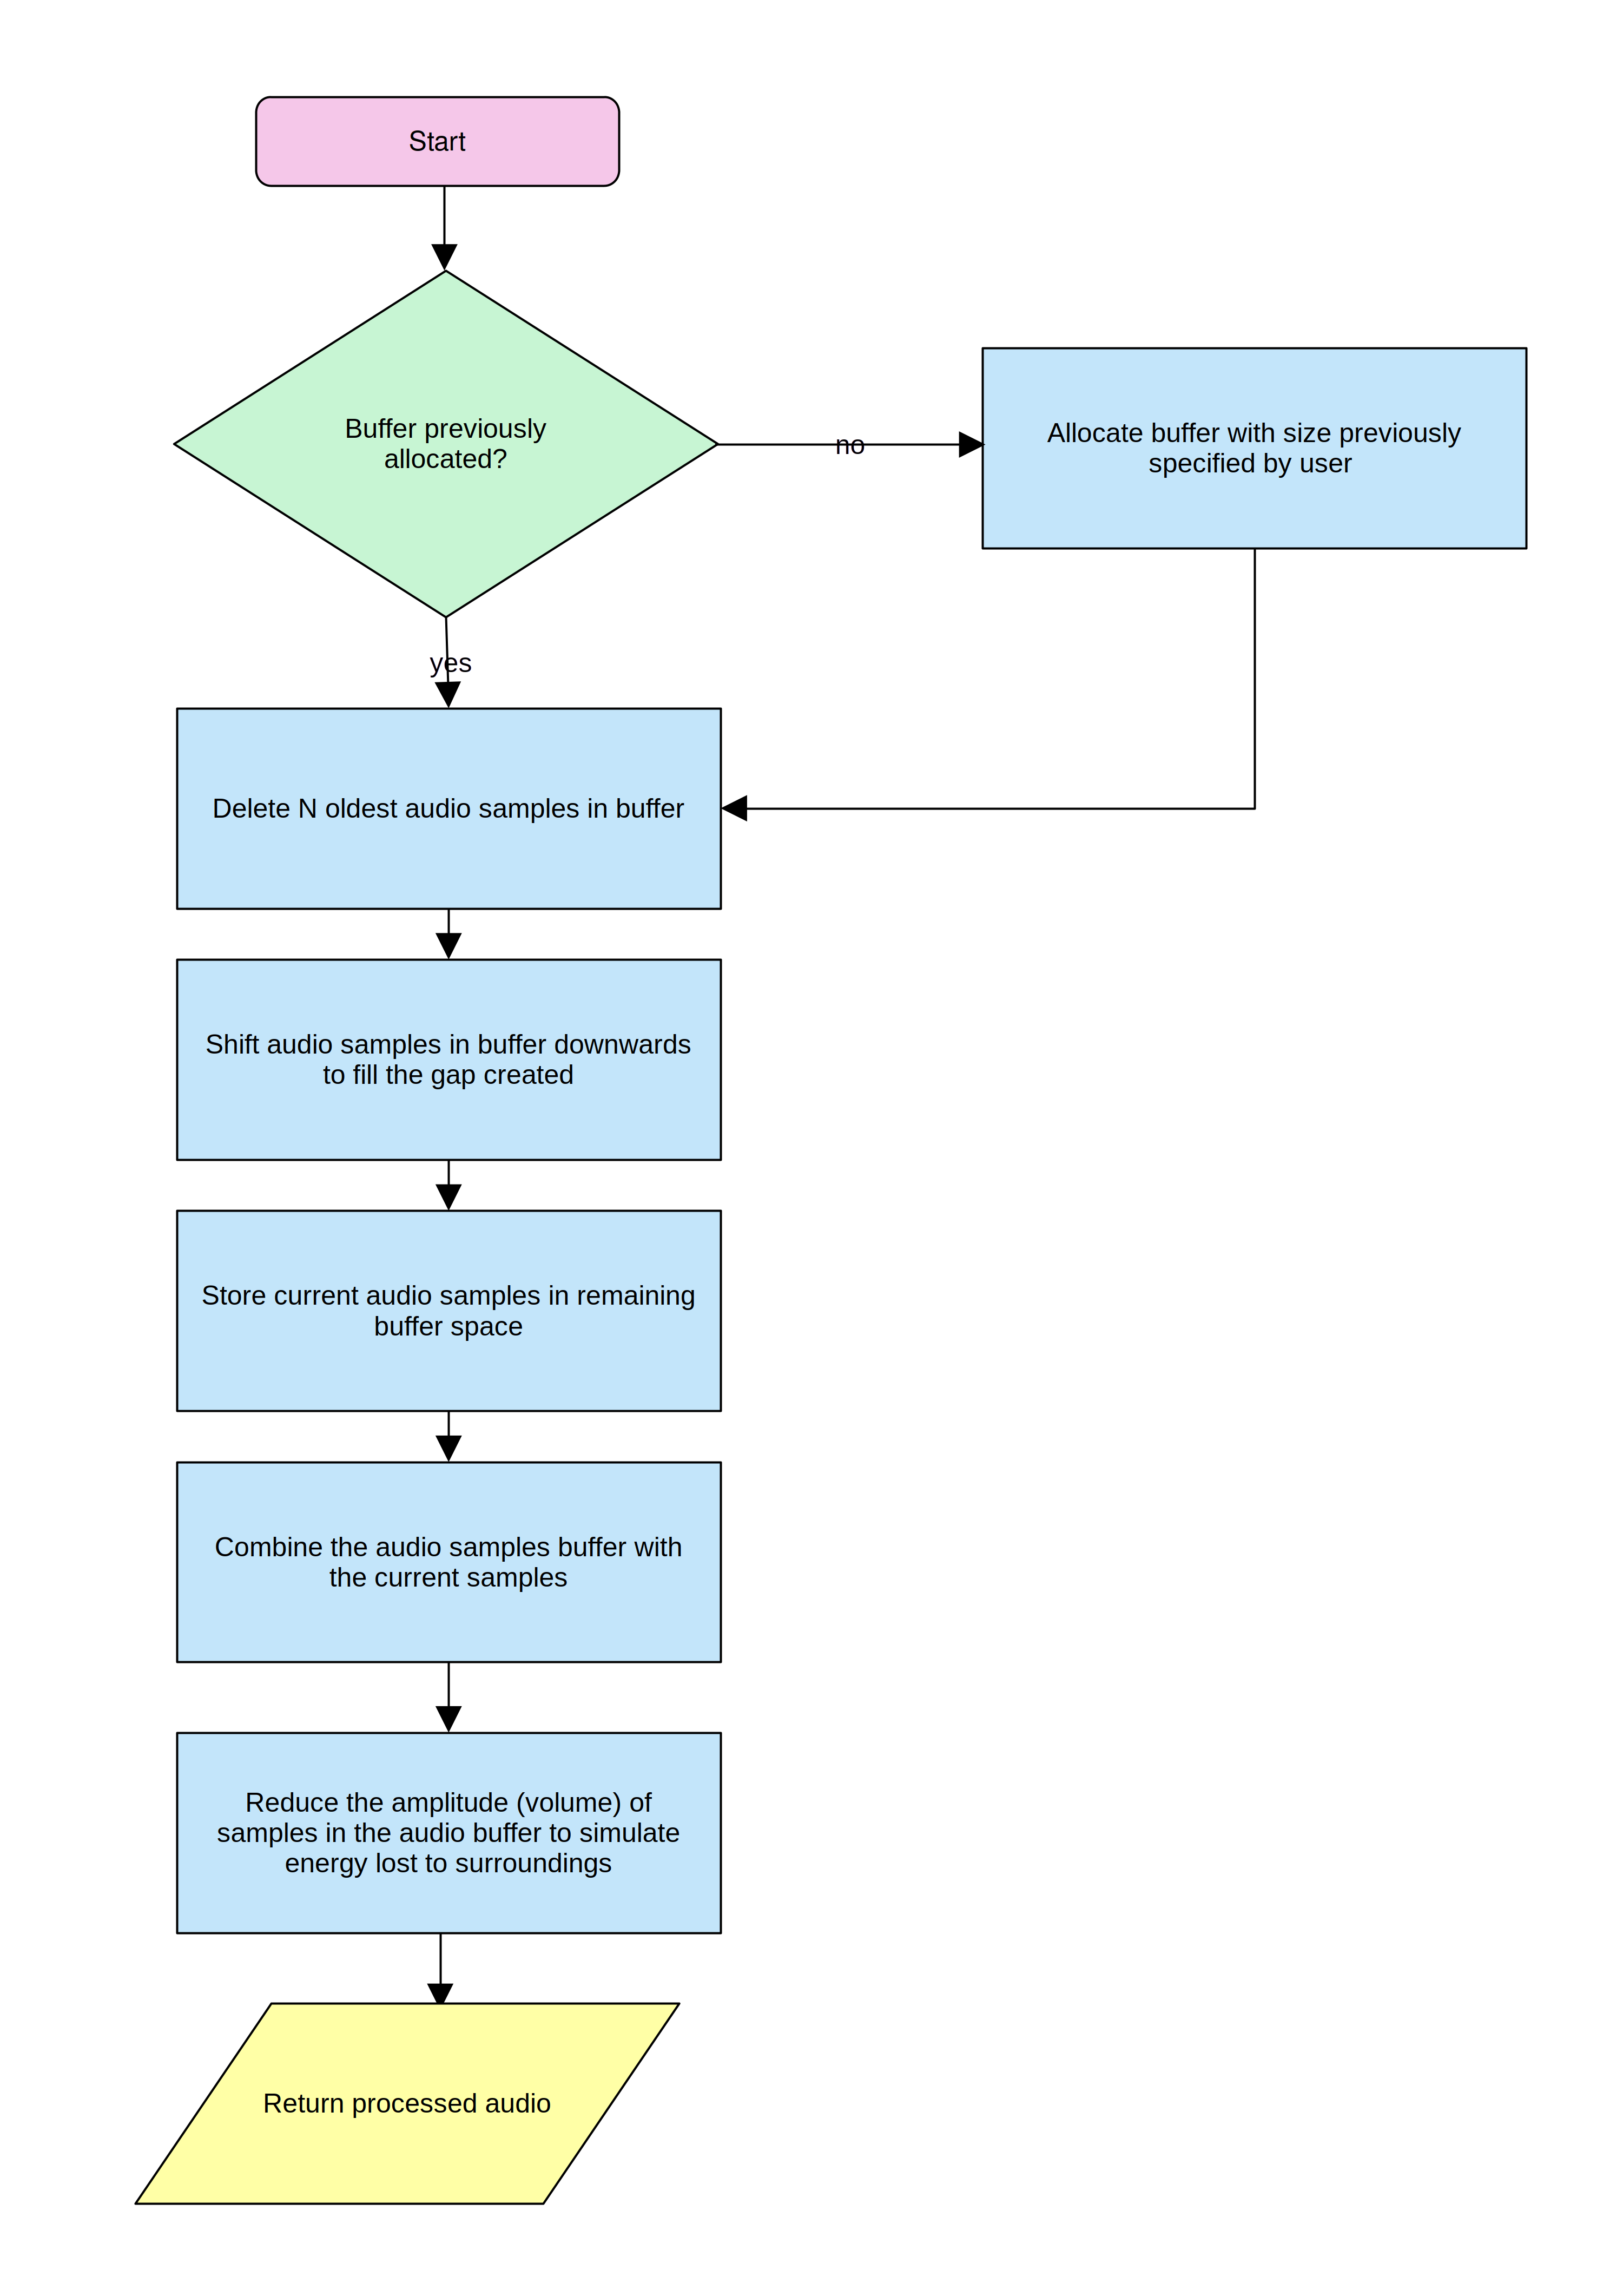
\includegraphics[width=14cm]{./echo flowchart.png}
	\caption{Flowchart for echo audio effect}
\end{figure}

\begin{figure}[H]
	\subsubsection{Volume}
	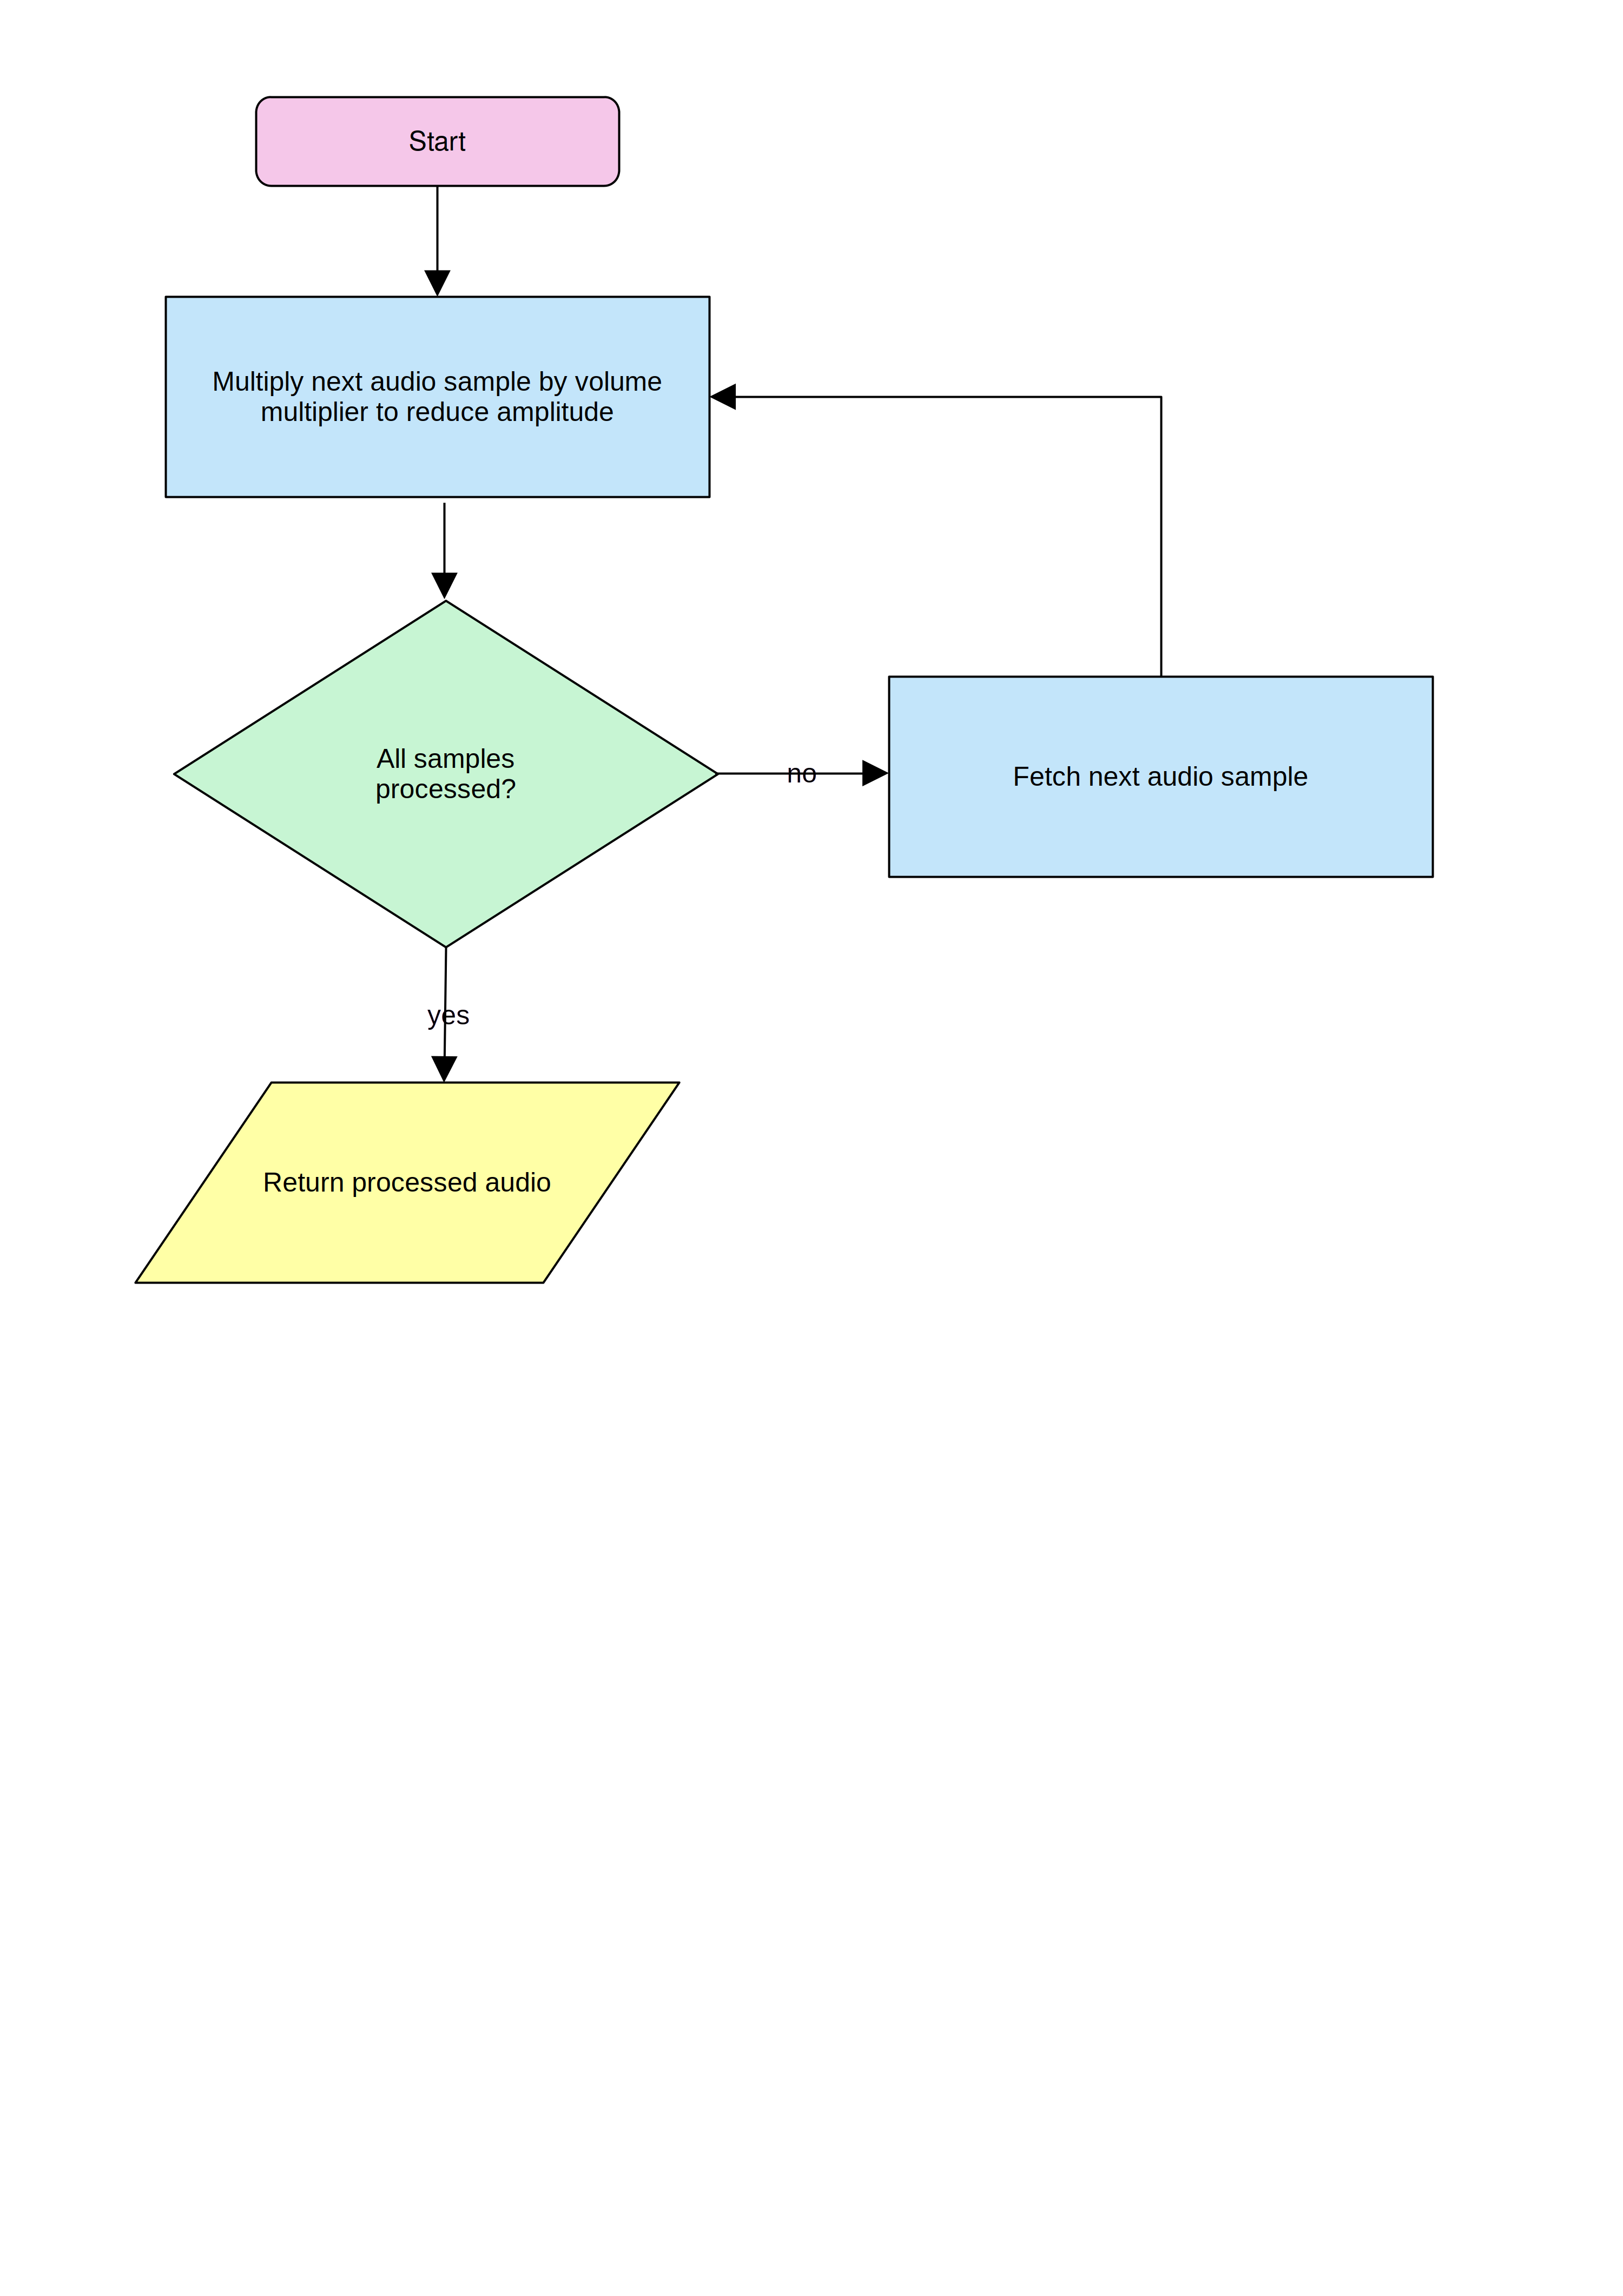
\includegraphics[width=14cm]{./volume flowchart.png}
	\caption{Flowchart for volume audio effect}
\end{figure}

\begin{figure}[H]
	\subsubsection{Noise}
	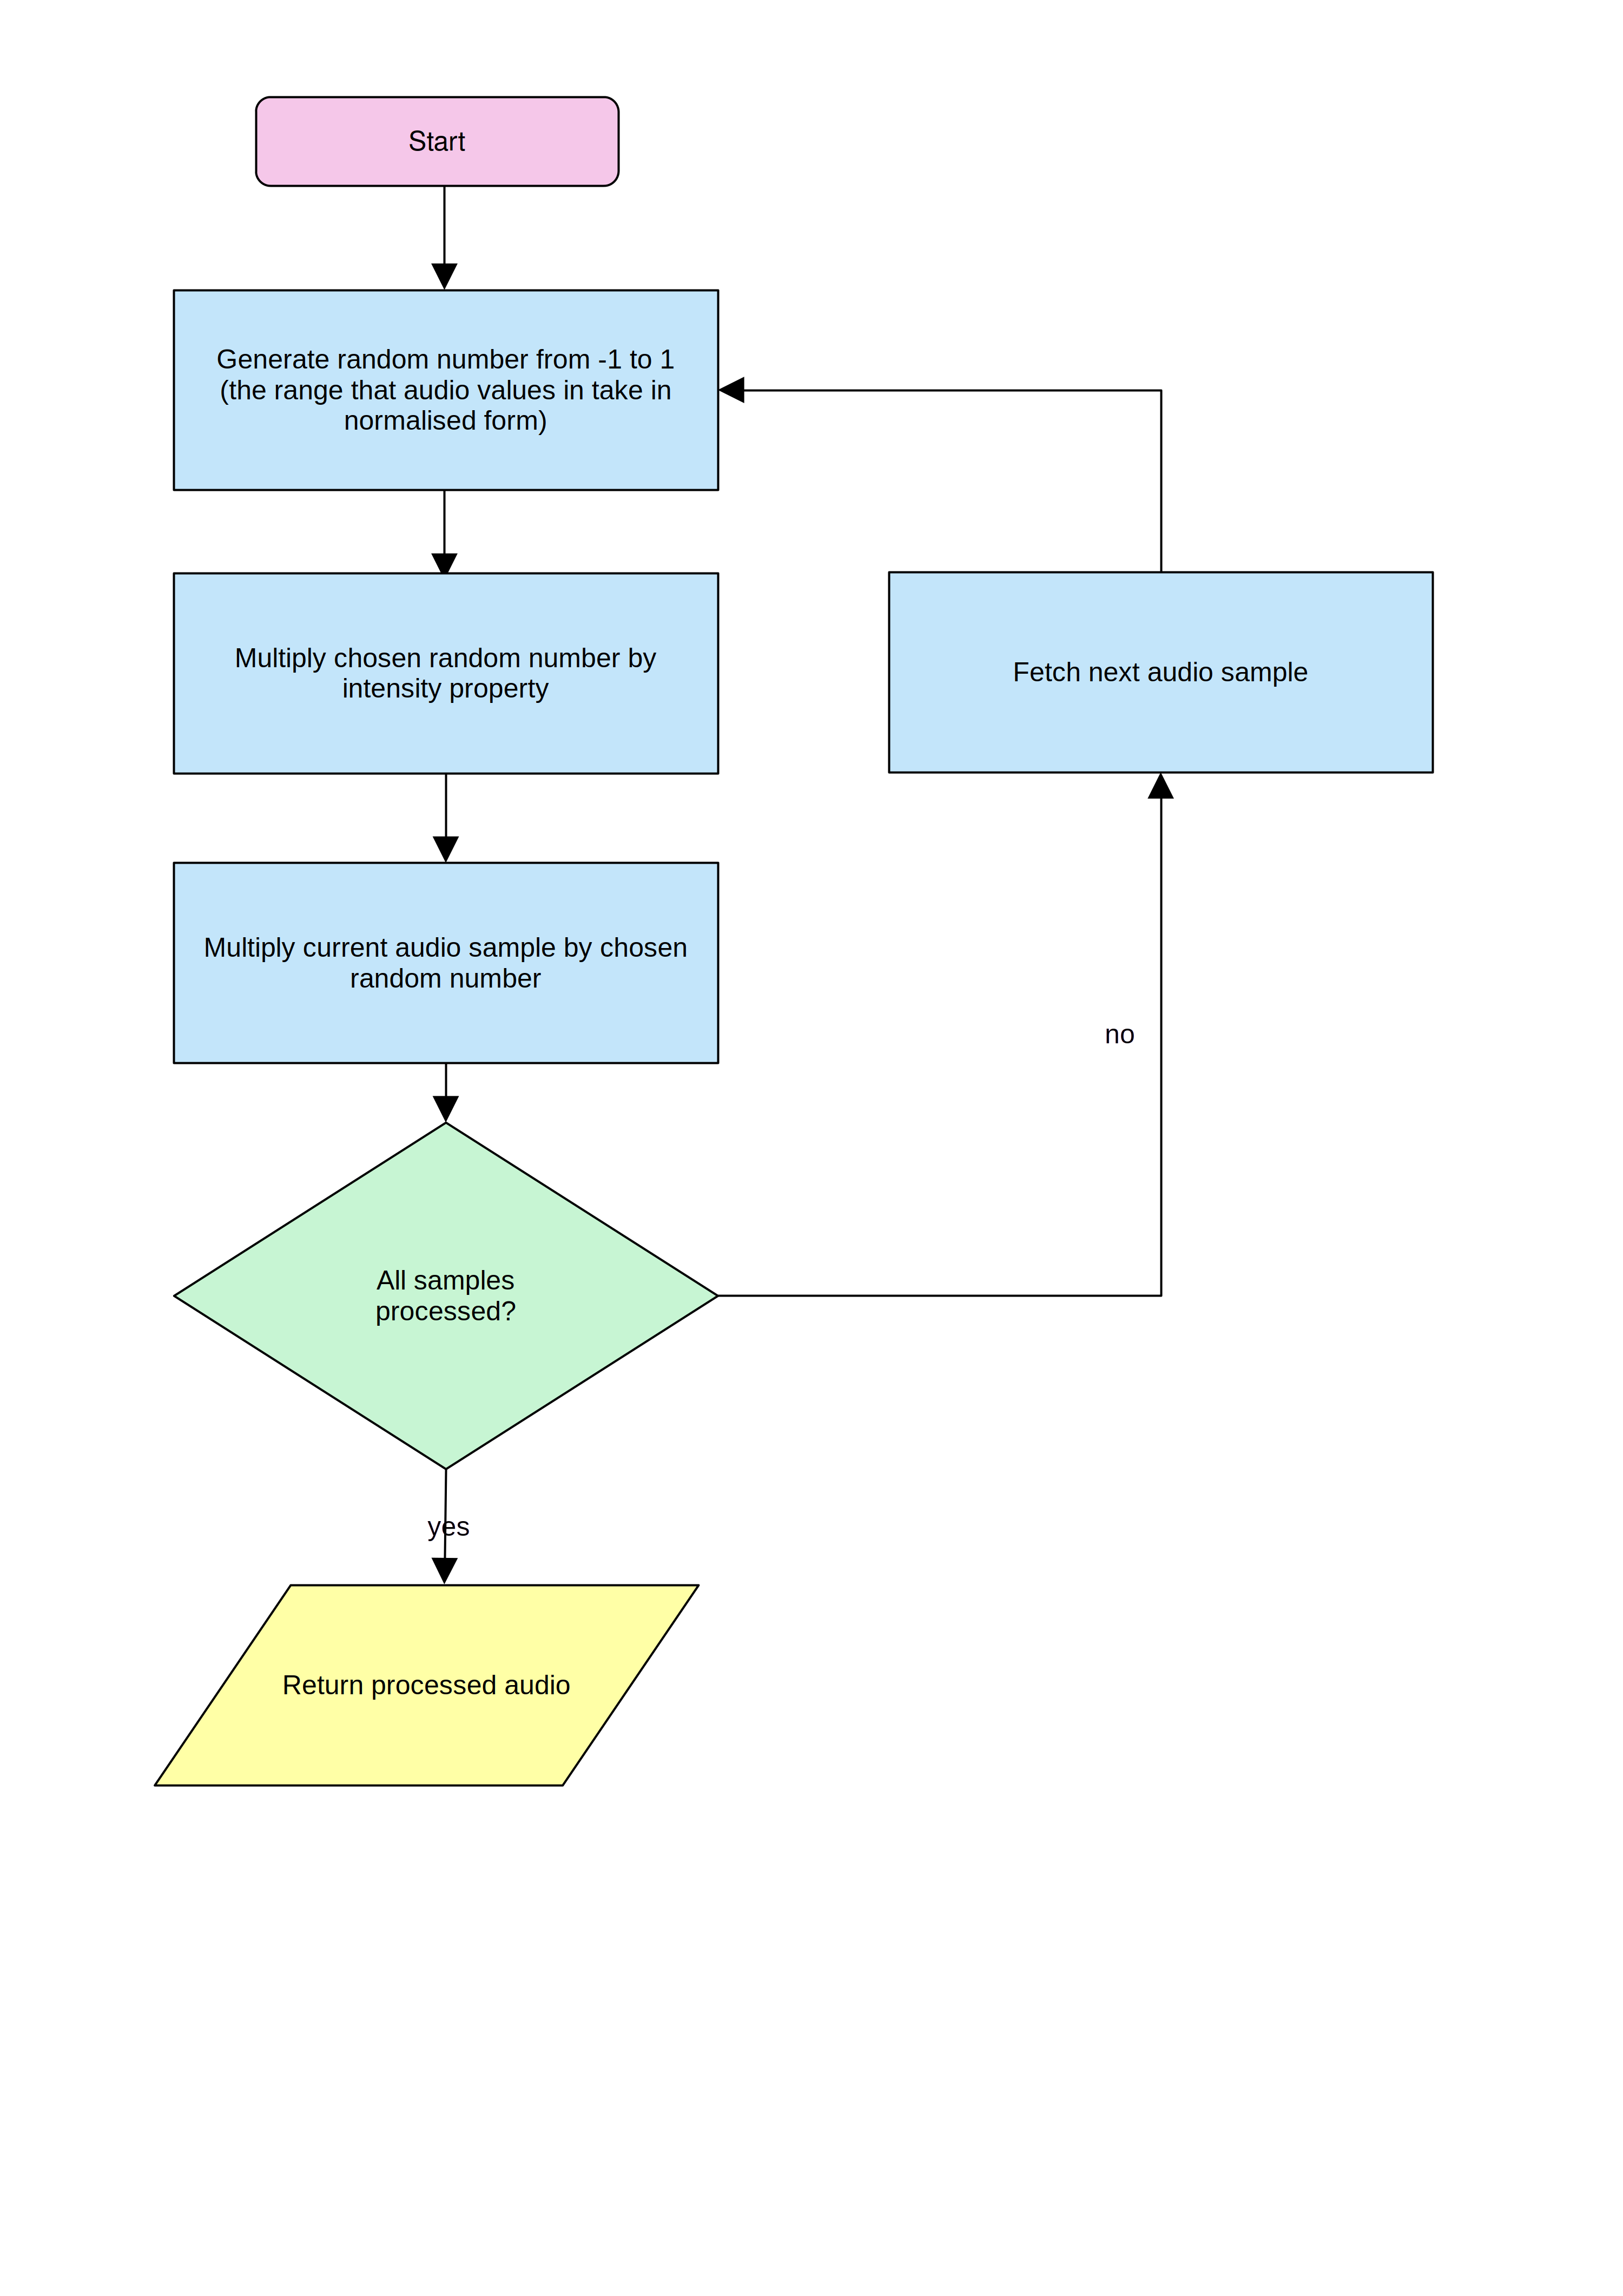
\includegraphics[width=14cm]{./noise flowchart.png}
	\caption{Flowchart for noise audio effect}
\end{figure}

\pagebreak
\subsection{Audio Visualisation and Fourier Algorithm}

\paragraph{} As can be seen in the equaliser flowchart, there is a need to perform both a Fourier Transform and an Inverse Fourier Transform on audio data in order to manipulate the audio in its frequency domain (i.e. to manipulate certain frequencies in isolation). In addition, as per the objectives outlined above, the program has a need to use this data to visualise the audio being played ("the user must be able to visualise the current audio being played in the frequency domain").

\paragraph{} Hence there is a need for pseudo-code to be designed to perform the three algorithms involved:
\begin{enumerate}
	\item A Fast Fourier Transform to convert incoming time-domain audio to its frequency-domain
	\item An algorithm that graphically displays this frequency-domain audio for the purposes of visualisation
	\item An Inverse Fast Fourier Transform to convert frequency-domain audio back to the time-domain
\end{enumerate}

\subsubsection{Cooley-Tukey FFT and IFFT Algorithm}

\paragraph{Summary of Fourier Analysis from Section 1}  Careful consideration of the problem in the analysis section revealed that acceptable performance could be achieved by using a Fast Fourier Transform (FFT), which used various mathematical techniques to reduce time complexity from \(O(N^2)\) to \(O(N\log{N})\), greatly reducing computational overhead. The most popular FFT algorithm, the "Cooley-Tukey"  FFT, was chosen, due to its use of recursion to both efficiently  and elegantly perform the computations required.

\paragraph{Comparing the FFT and IFFT}
It should be stressed that there is very little difference between performing a "normal" Fast Fourier Transform using the Cooley-Tukey algorithm and an \textit{inverse} Fast Fourier Transform. For this reason, I have decided to combine the two into a single function to eliminate as much code duplication as possible.

\pagebreak
\paragraph{Pseudo-code implementation of algorithm}
\begin{minted}{ada}
-- Converts an array of floats (i.e. the audio samples) into an array of complex numbers
-- by using 0 for the imaginary parts. We must check the incoming data is a power of 2
-- as later code that uses the results of this computation (i.e. the FFT) depends on this.
function convert_samples_to_complex_form(samples: array of float) -> array of complex:
	if size of samples is not a power of 2:
		raise error "FFT data has invalid size"

	complex_samples := new array of complex with size equal to size of samples
	for each sample in samples:
		append (sample, 0.0) as a complex number to complex_samples

	return complex_samples

-- Performs both either an FFT or an IFFT recursively by diving the data into two
-- until the trivial base case is reached
function do_fft(input: reference to array of complex, mode: Mode):
	N := size of input
	if N <= 1:
		return

	-- Split data by even and odd indices
	even := new array of complex with size N/2
	odd := new array of complex with size N/2
	for i from 0 to N/2 - 1:
		even[i] := input[2*i]
		odd[i] := input[2*i + 1]

	-- Perform FFT / IFFT recursively on even and odd halves
	do_fft(even, mode)
	do_fft(odd, mode)

	for k from 0 to N/2 - 1:
		-- Perform FFT calculation by manipulating audio sample in the complex plane
		-- as per the formal defition (see analysis section)
		sign := if mode is Normal then -1.0 else 1.0
		t := polar(1.0, sign * 2.0 * PI * k / N) * odd[k]
		input[k] := even[k] + t
		input[k + N/2] := even[k] - t

-- Example code for using FFT
incoming_audio = fetch_upcoming_audio_data_from_buffer()
complex_audio = convert_samples_to_complex_form(incoming_audio)
do_fft(complex_audio, Mode::Normal)

-- (calculations on frequency domain, including visualisation, performed here)

-- Convert back to time domain (example code using IFFT)
do_fft(fft_result, Mode::Inverse)
final_audio = discard_imaginary_parts_of_complex_array(complex_audio)
submit_audio_to_speakers(final_audio)
\end{minted}

\pagebreak
\subsubsection{Visualisation Algorithm}

\paragraph{Interpreting the results of an FFT}
After an FFT has been performed, the resultant frequency-domain data needs to be visualised. The data returned from an FFT is an array of complex numbers where each index corresponds to a particular range of frequencies. The amplitude of these frequencies is just the magnitude of the complex number at that index. For example, index 12 might correspond to frequencies from 100 Hz to 130 Hz, and the magnitude of the complex number at fft\_array[12] would be the amplitude.

\paragraph{}
The range of frequencies each element in the FFT data represents is called the "frequency resolution", whereby:
\[
\text{frequency resolution} = \frac{\text{frequency of incoming audio}}{\text{number of samples in audio provided to FFT algorithm}}
\]

\paragraph{}
Hence for any given index in the array, the minimum frequency it represents is given by:
\[
	\text{min frequency} = \text{index in the array} \times \text{frequency resolution}
\]

\paragraph{}
The visualisation I have chosen is a bar chart, where the x-axis represents frequency and the y-axis represents amplitude. Each bar can be said to have:
\begin{itemize}
	\item a minimum frequency
	\item a maximum frequency
	\item an amplitude
\end{itemize}
Hence an algorithm is needed to convert the incoming FFT frequency-domain data into the above format for later rendering. The minimum and maximum frequencies can be derived from the equations above.

\paragraph{Using a non-uniform scale for frequency}
The human ear does not perceive frequencies in a linear fashion. In other words, if one adds 500 Hz to a sound-wave repeatedly, the "jump" in pitch will not always sound the same.  This is because human-hearing follows a roughly logarithmic scale when it comes to detecting frequencies. This represents a problem as using a uniform, linear scale on the visualisation bar chart, whilst mathematically correct, will not sound plausible to the ear. Instead, the x-axis (frequency) for the bar chart must be adjusted so that, relative to the human ear, each bar represents roughly the same jump in \textit{perceived} pitch. The most suitable scale for this is the "Bark scale", where "equal distances correspond with perceptually equal distances" as described above. A frequency can be converted into its Bark equivalent using a simple formula:
\[
\text{Bark} = 13 \arctan(0.00076 \times \text{frequency}) + 3.5 \arctan ((\text{frequency} / 7500)^2)
\]

\paragraph{Using a non-uniform scale for amplitude}
Just like with frequency, the human ears perceive amplitude logarithmically too. If a sound-wave has twice the frequency, it will not necessarily sound twice as loud. Thus the y-axis of the bar chart must be adjusted to reflect the \textit{perceived} loudness. A good  approximation is to take each amplitude and log it to base 10.

\paragraph{Ignoring inaudible sounds}
The human ear cannot hear sounds below 20 Hz or above 20,000 Hz. These frequencies should therefore be ignored in the visualisation, and hence the algorithm should be able to reject frequencies outside a specified frequency,

\pagebreak
\begin{minted}{ada}
function hertz_to_bark_scale(hertz: float) -> float:
	return 13.0 * arctan(0.00076 * hertz) + 3.5 * arctan((hertz / 7500.0) * (hertz / 7500.0))

-- GroupSettings is a data structure consiting of the number of samples ("buckets") provided to the FFT,
-- the frequency of the incoming audio, and the minimum and maximum  acceptable frequencies.
function convert_fft_to_bar_chart_format(fft: array of complex, group_settings: GroupingSettings) -> array of FrequencyRange:

	-- Work out frequency resolution
	n_samples := size of fft
	frequency_resolution := group_settings.frequency / n_samples

	-- Work out min and max frequencies in Bark scale and distance between "buckets"
	minimum_frequency_bark := hertz_to_bark_scale(group_settings.minimum_audible_frequency)
	maximum_frequency_bark := hertz_to_bark_scale(group_settings.maximum_audible_frequency)
	bark_distance := (maximum_frequency_bark - minimum_frequency_bark) / group_settings.n_buckets

	buckets := new array of float with size equal to group_settings.n_buckets, initialized with zeros

	-- The FFT is symmetrical (because audio data lies only on the real axis), so we actually only  need
	-- to visualise the first half of it
	for i from 0 to (n_samples/2 - 1):
		frequency := i * frequency_resolution
		if frequency >= group_settings.minimum_audible_frequency
		  and frequency <= group_settings.maximum_audible_frequency:

			-- Use Bark scale conversion to work out location of "bar" in bar chart
			bark_frequency := HertzToBarkScale(frequency)
			index := (bark_frequency - minimum_frequency_bark) / bark_distance

			if index < size of buckets:
				-- Calculate amplitude of frequency (i.e. the magnitude of the complex number)
				-- Add this to the height of the bar at this point in the bar chart
				buckets[index] += absolute value of fft[i]

	-- Work out maximum amplitude in bar chart
	max_magnitude := 0.0
	for each bucket in buckets:
		if bucket > max_magnitude:
			max_magnitude := bucket

	-- Scale magnitudes logarithmically
	for each bucket in buckets:
		bucket := logarithm base 10 of (1.0 + bucket / max_magnitude)

	-- Convert bucket array (raw bar chart data) into a more usable format
	ranges := new array of FrequencyRange with size equal to size of buckets
	for i from 0 to size of buckets - 1:
		lower_freq := minimum_frequency_bark + (i + 0.0) * bark_distance
		upper_freq := maximum_frequency_bark + (i + 1.0) * bark_distance

		-- Convert back to Hertz scale
		lower_freq := 0.5 + 600.0 * sinh(lower_freq / 6.0)
		upper_freq := 0.5 + 600.0 * sinh(upper_freq / 6.0)

		ranges[i] := FrequencyRange {
			min_frequency: integer part of lower_freq,
			max_frequency: integer part of upper_freq,
			magnitude: buckets[i]
		}

	return ranges
\end{minted}
\pagebreak
\begin{minted}{ada}
function draw_bar_chart(bars: array of FrequencyRange):
	draw_screen_background()

	-- Find max magnitude
	max_magnitude := 0.0
	for i from 0 to size of bars - 1:
		if (bars[i].magnitude > max_magnitude)
			max_magnitude = bars[i].magnitude

	-- Work out scaling
	bar_width := screen_width / (size of bars)
	bar_height_scale := screen_heigh / max_magnitude

	for i from 0 to size of bars - 1:
		bar_height = bars[i].magnitude * bar_height_scale
		draw_rectangle(
			x: i * bar_width,
			y: 0,
			width: bar_width,
			height: bar_height
		)
\end{minted}

\pagebreak

\pagebreak
\subsection{Program GUI}

\paragraph{}
The user will interact with the program using a GUI. In order to maximise the potential user-base, I have decided to use a popular C++ GUI library called "wxWidgets", which allows for the creation of GUIs using a singular code-base for Windows, Linux and MacOS, amongst others.

\subsubsection{GUI "screens"}
The user will navigate through a variety of "screens" in order to use the program. The GUI flow can be modelled as followed:
\begin{itemize}
	\item When the program starts, the user must chose to either load an existing playlist (see "Audio Data and Playback"), or create a new one - this is the "choice screen".
	\item Should the user chose to create a playlist, a new "screen" will be displayed where they can append audio files on the system to a playlist, before saving it.
	\item Returning back to the initial "choice screen", the user will then chose to load their existing playlist, or optionally create another one for later use.
	\item After a playlist has been selected, the main "playback screen" will be displayed. Audio playback will begin.
	\item The user can view the current audio visualisation, as well as audio playback progress.
	\item A menu will allow the user to configure the current playback and visualisation, such as by adding new audio effects or changing the visualisation settings.
	\item A separate "screen" can be displayed allowing the user to view current audio effects.
	\item In this screen, if a user chooses to edit a current audio effect, a new screen will be displayed, showing the various options one can adjust.
\end{itemize}

\paragraph{Summary of "screens"}
\begin{itemize}
	\item "Choice" screen (create new playlist or load existing one)
	\item "Create playlist" screen
	\item "Playback" screen
	\item "Effects list" screen
	\item "Edit effect" screen
\end{itemize}

\paragraph{Popups}
Minor tasks such as  selecting a new song from a playlist or modifying visualisation settings will be handled with popup dialogue menus.

\begin{figure}[H]
	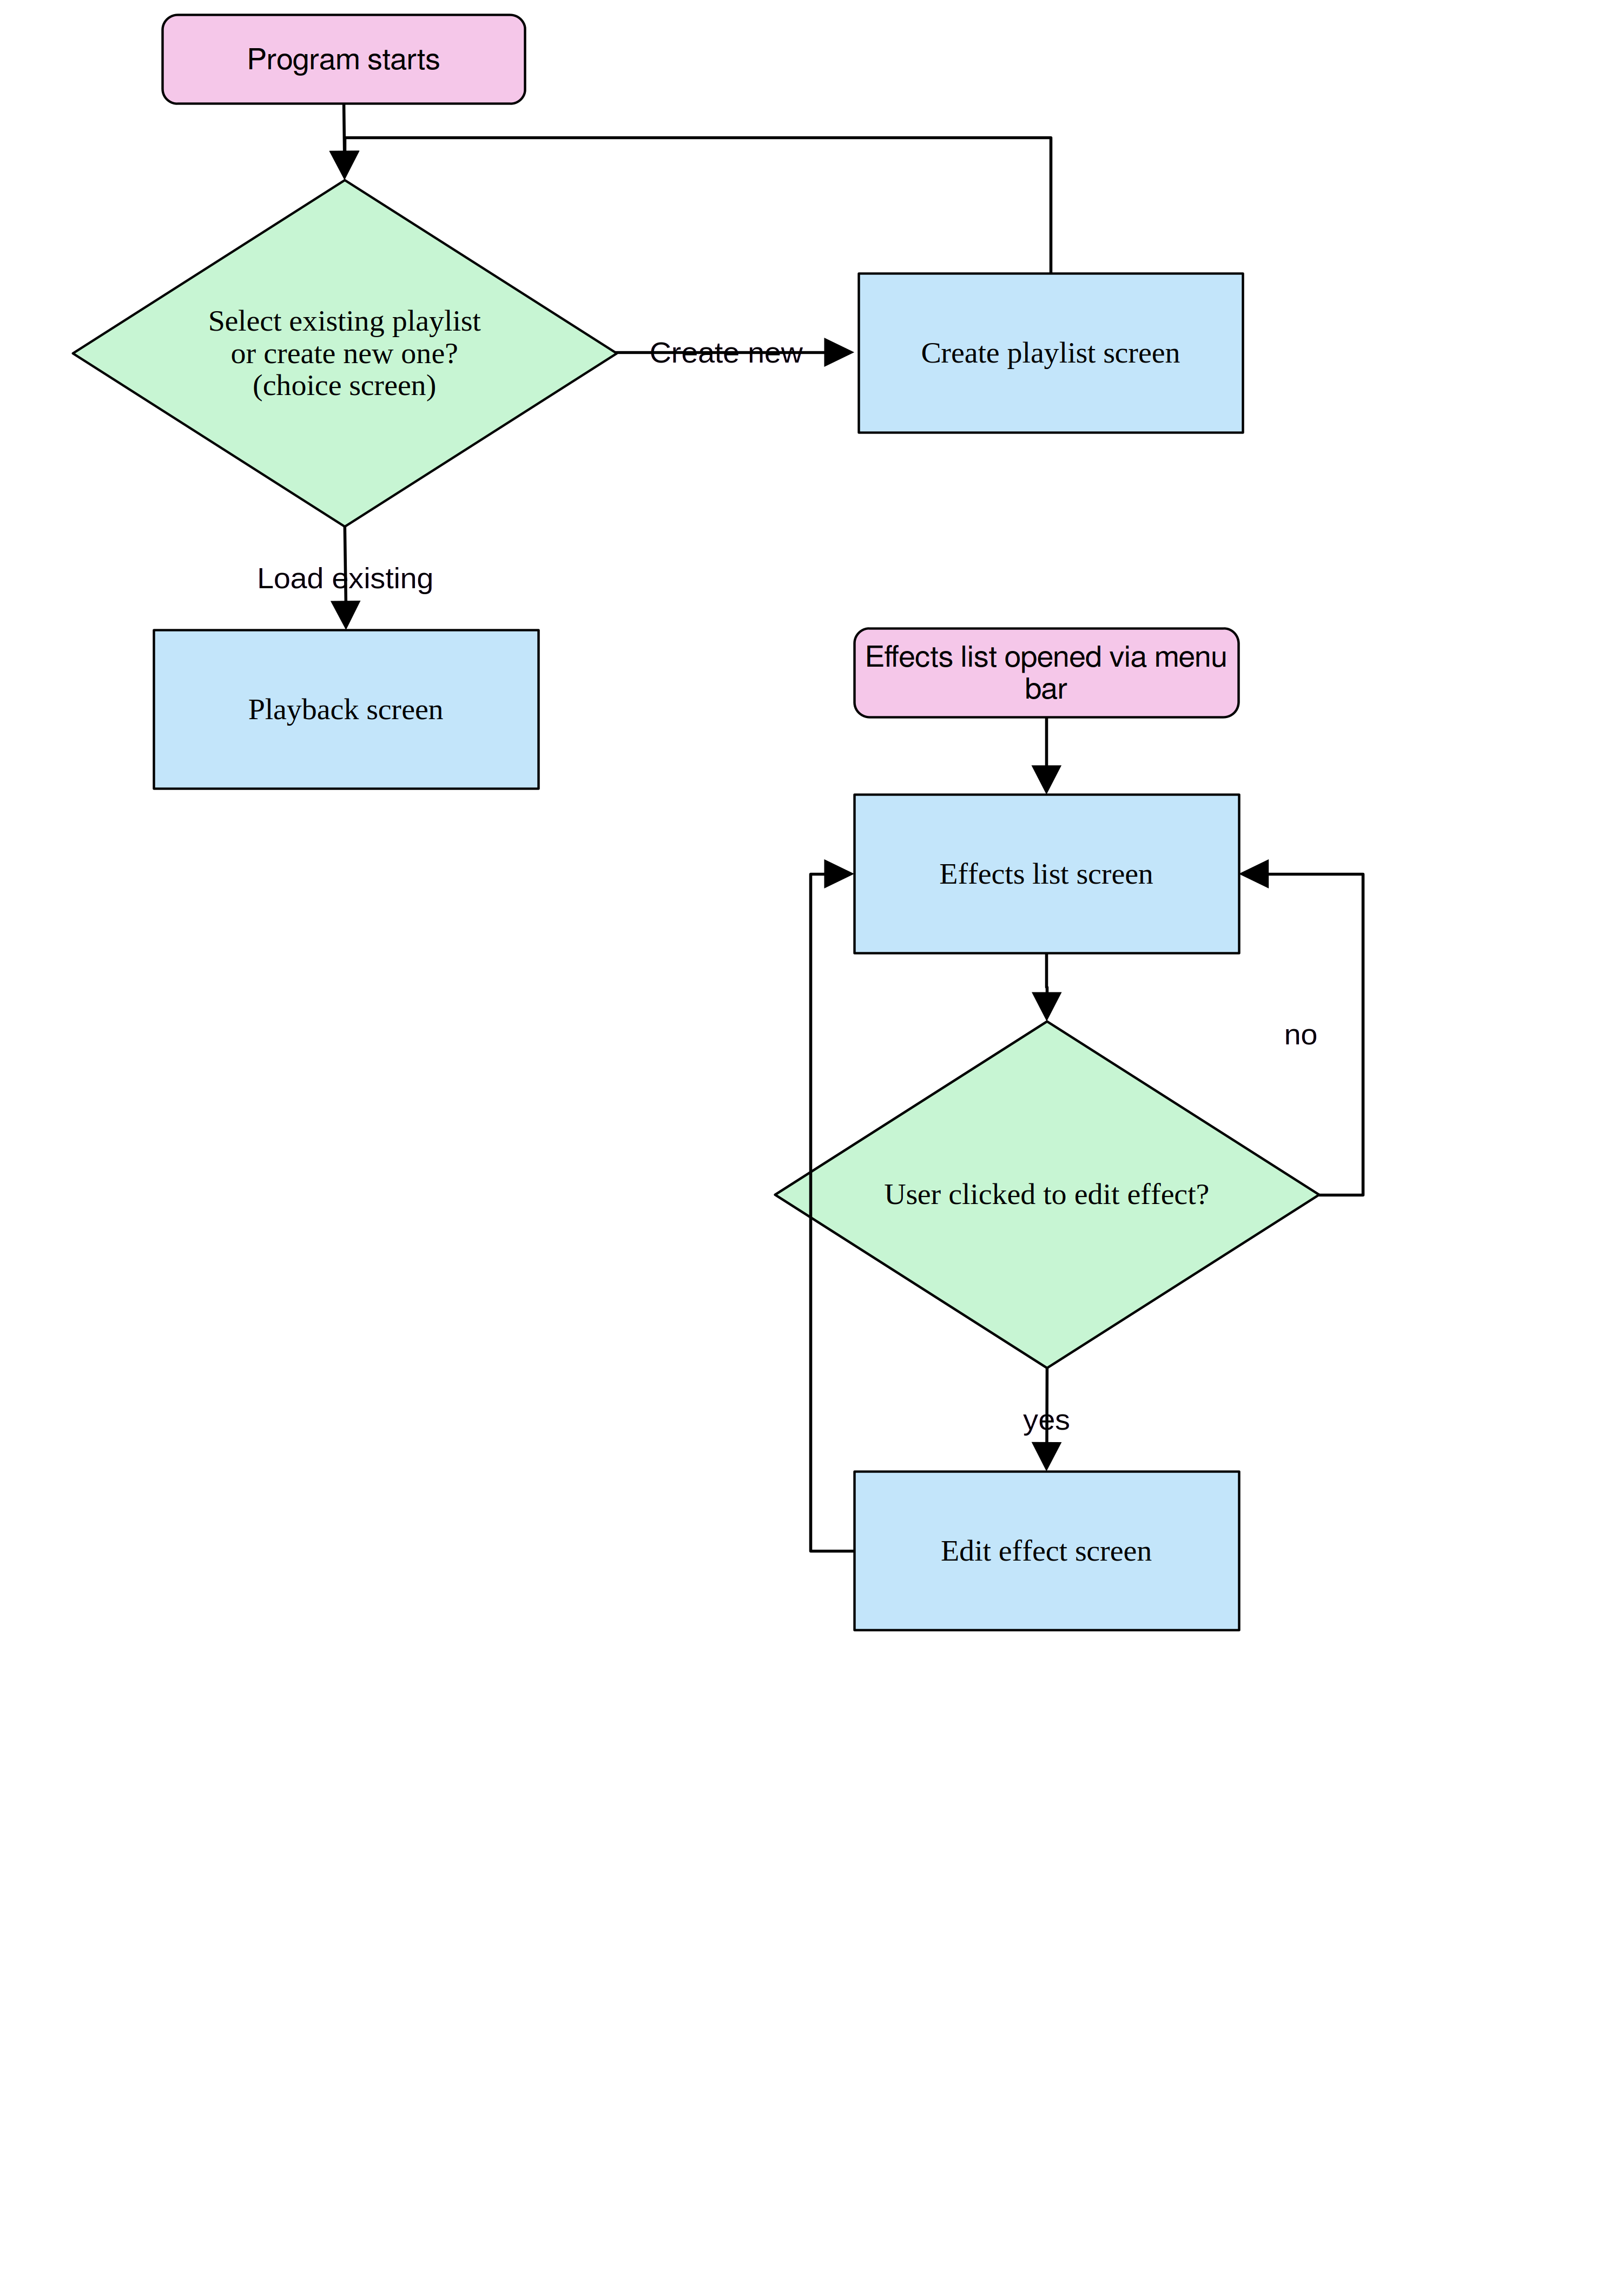
\includegraphics[width=14cm]{./gui flow.png}
	\caption{GUI flow for program }
\end{figure}

\subsubsection{GUI Wireframes}

\begin{figure}[H]
	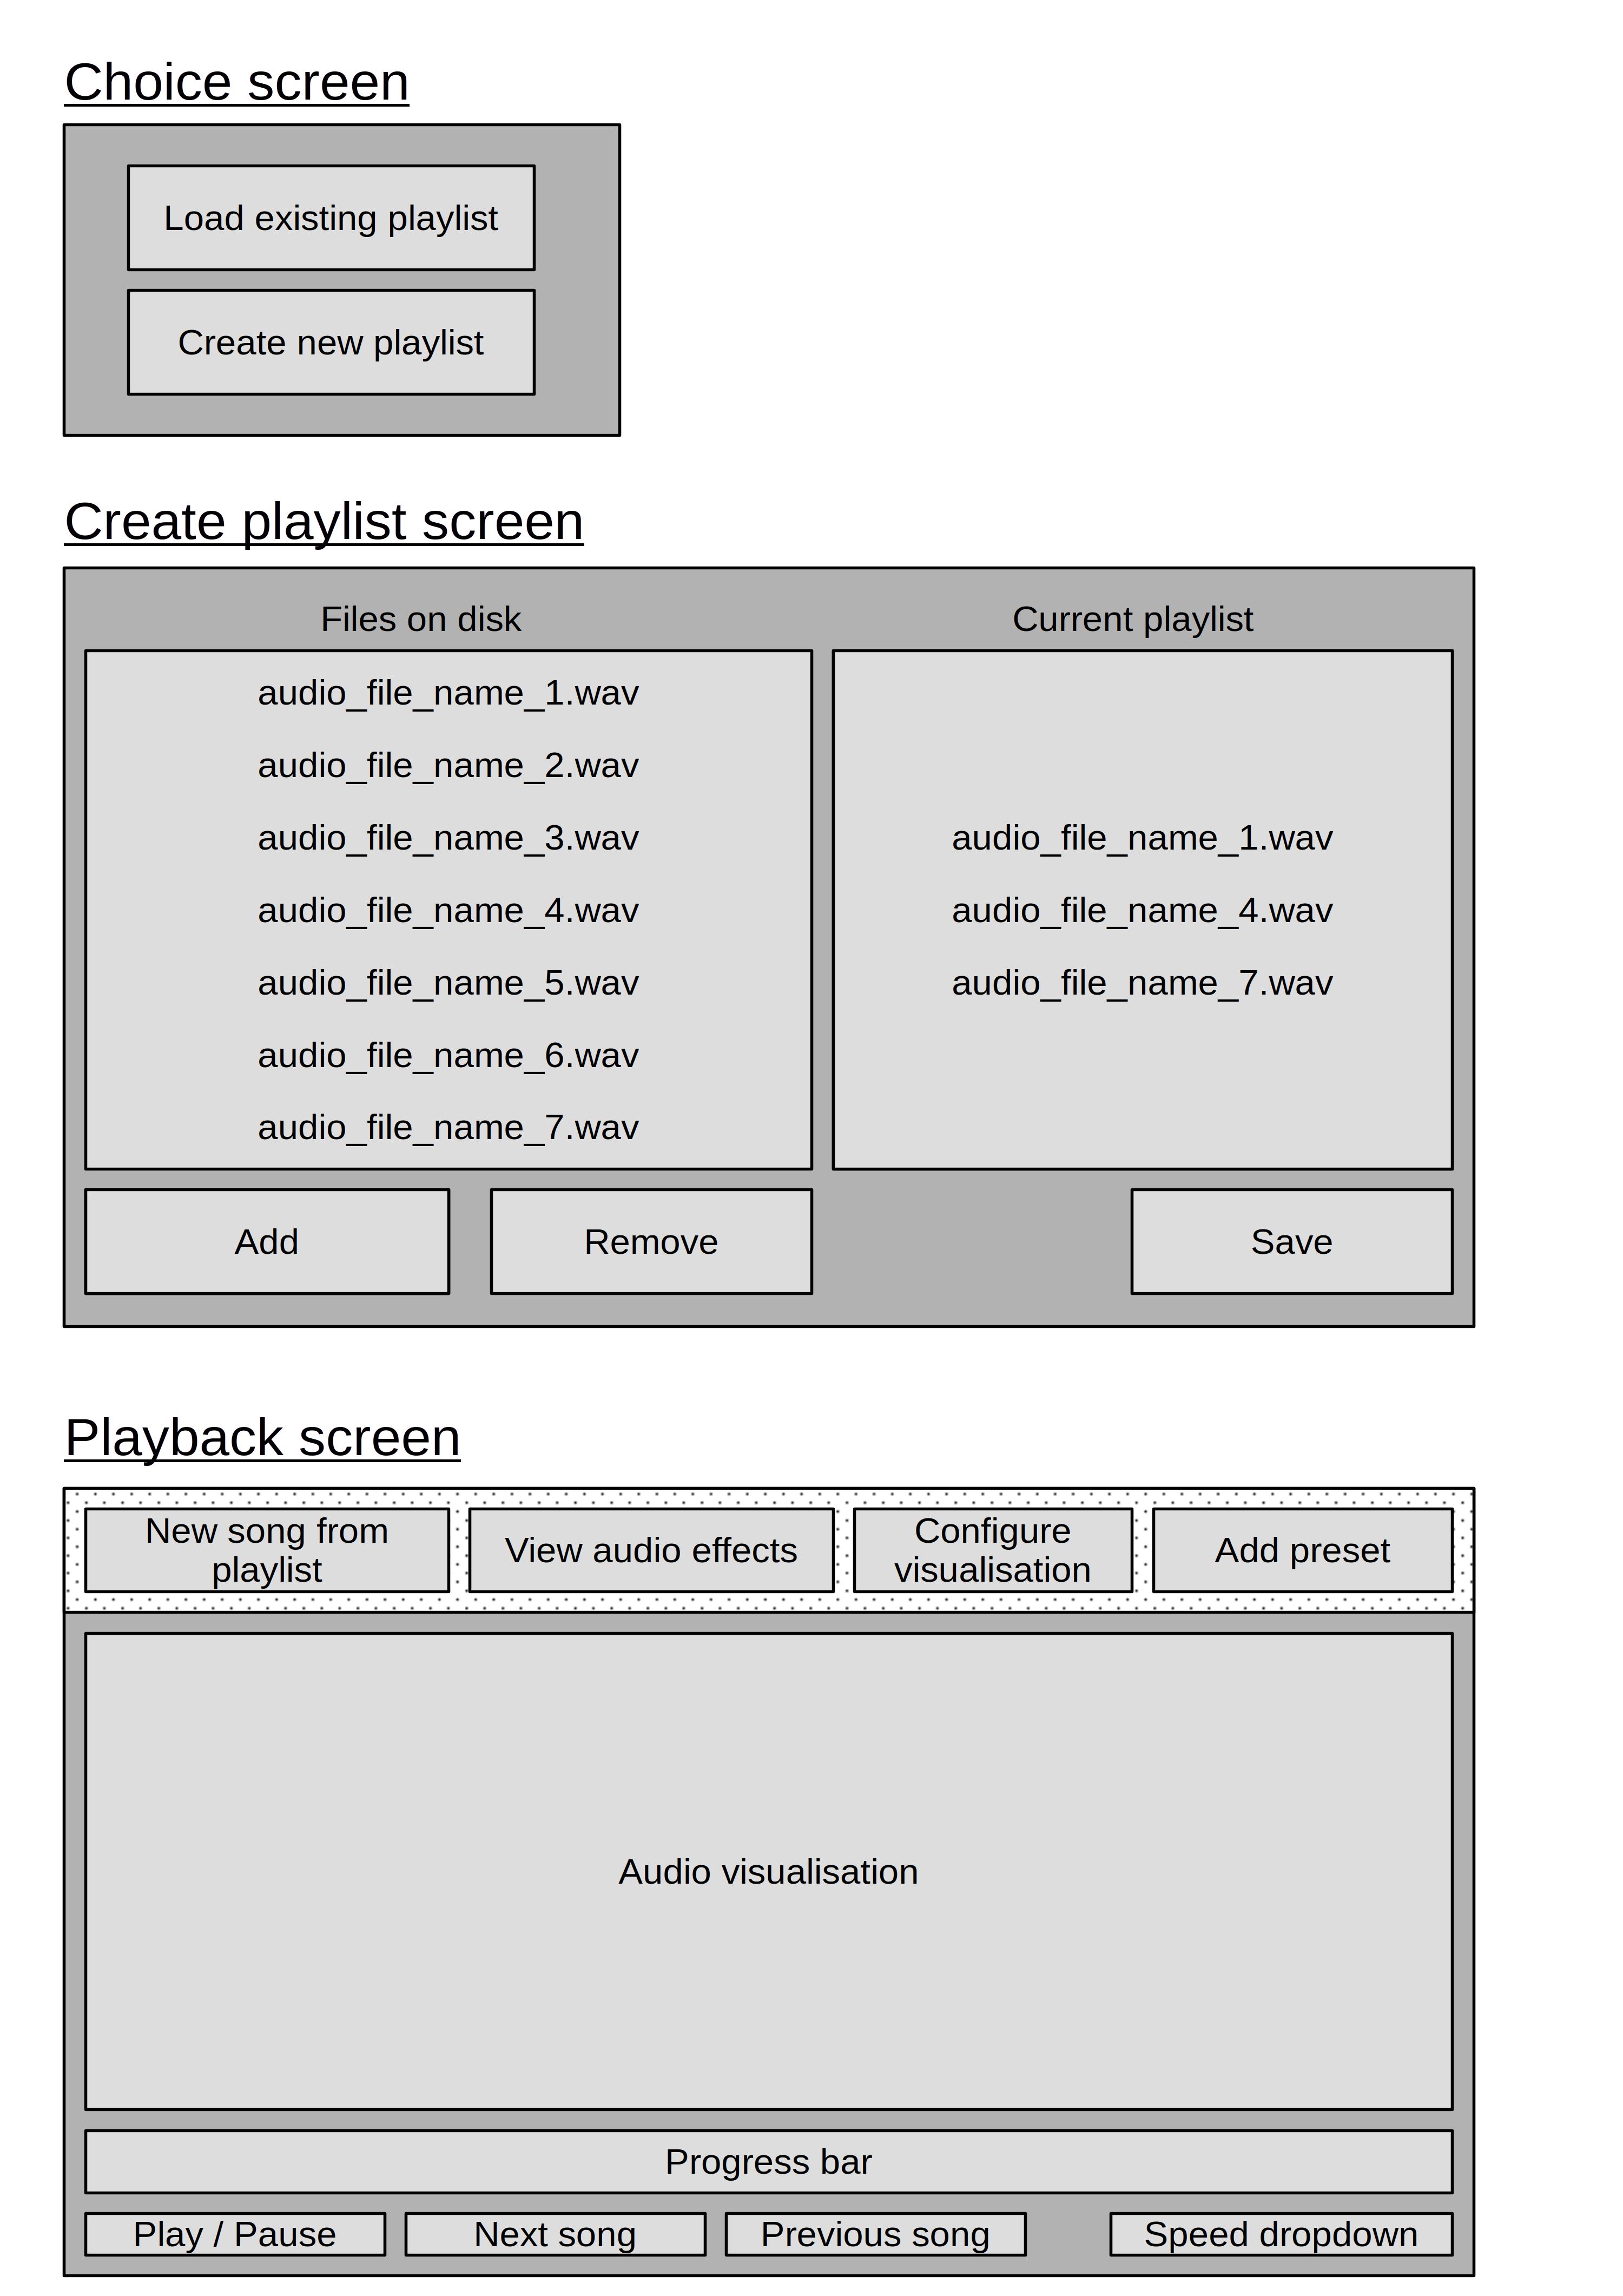
\includegraphics[width=14cm]{./gui wireframes one.png}
	\caption{GUI wireframes for main windows }
\end{figure}

\begin{figure}[H]
	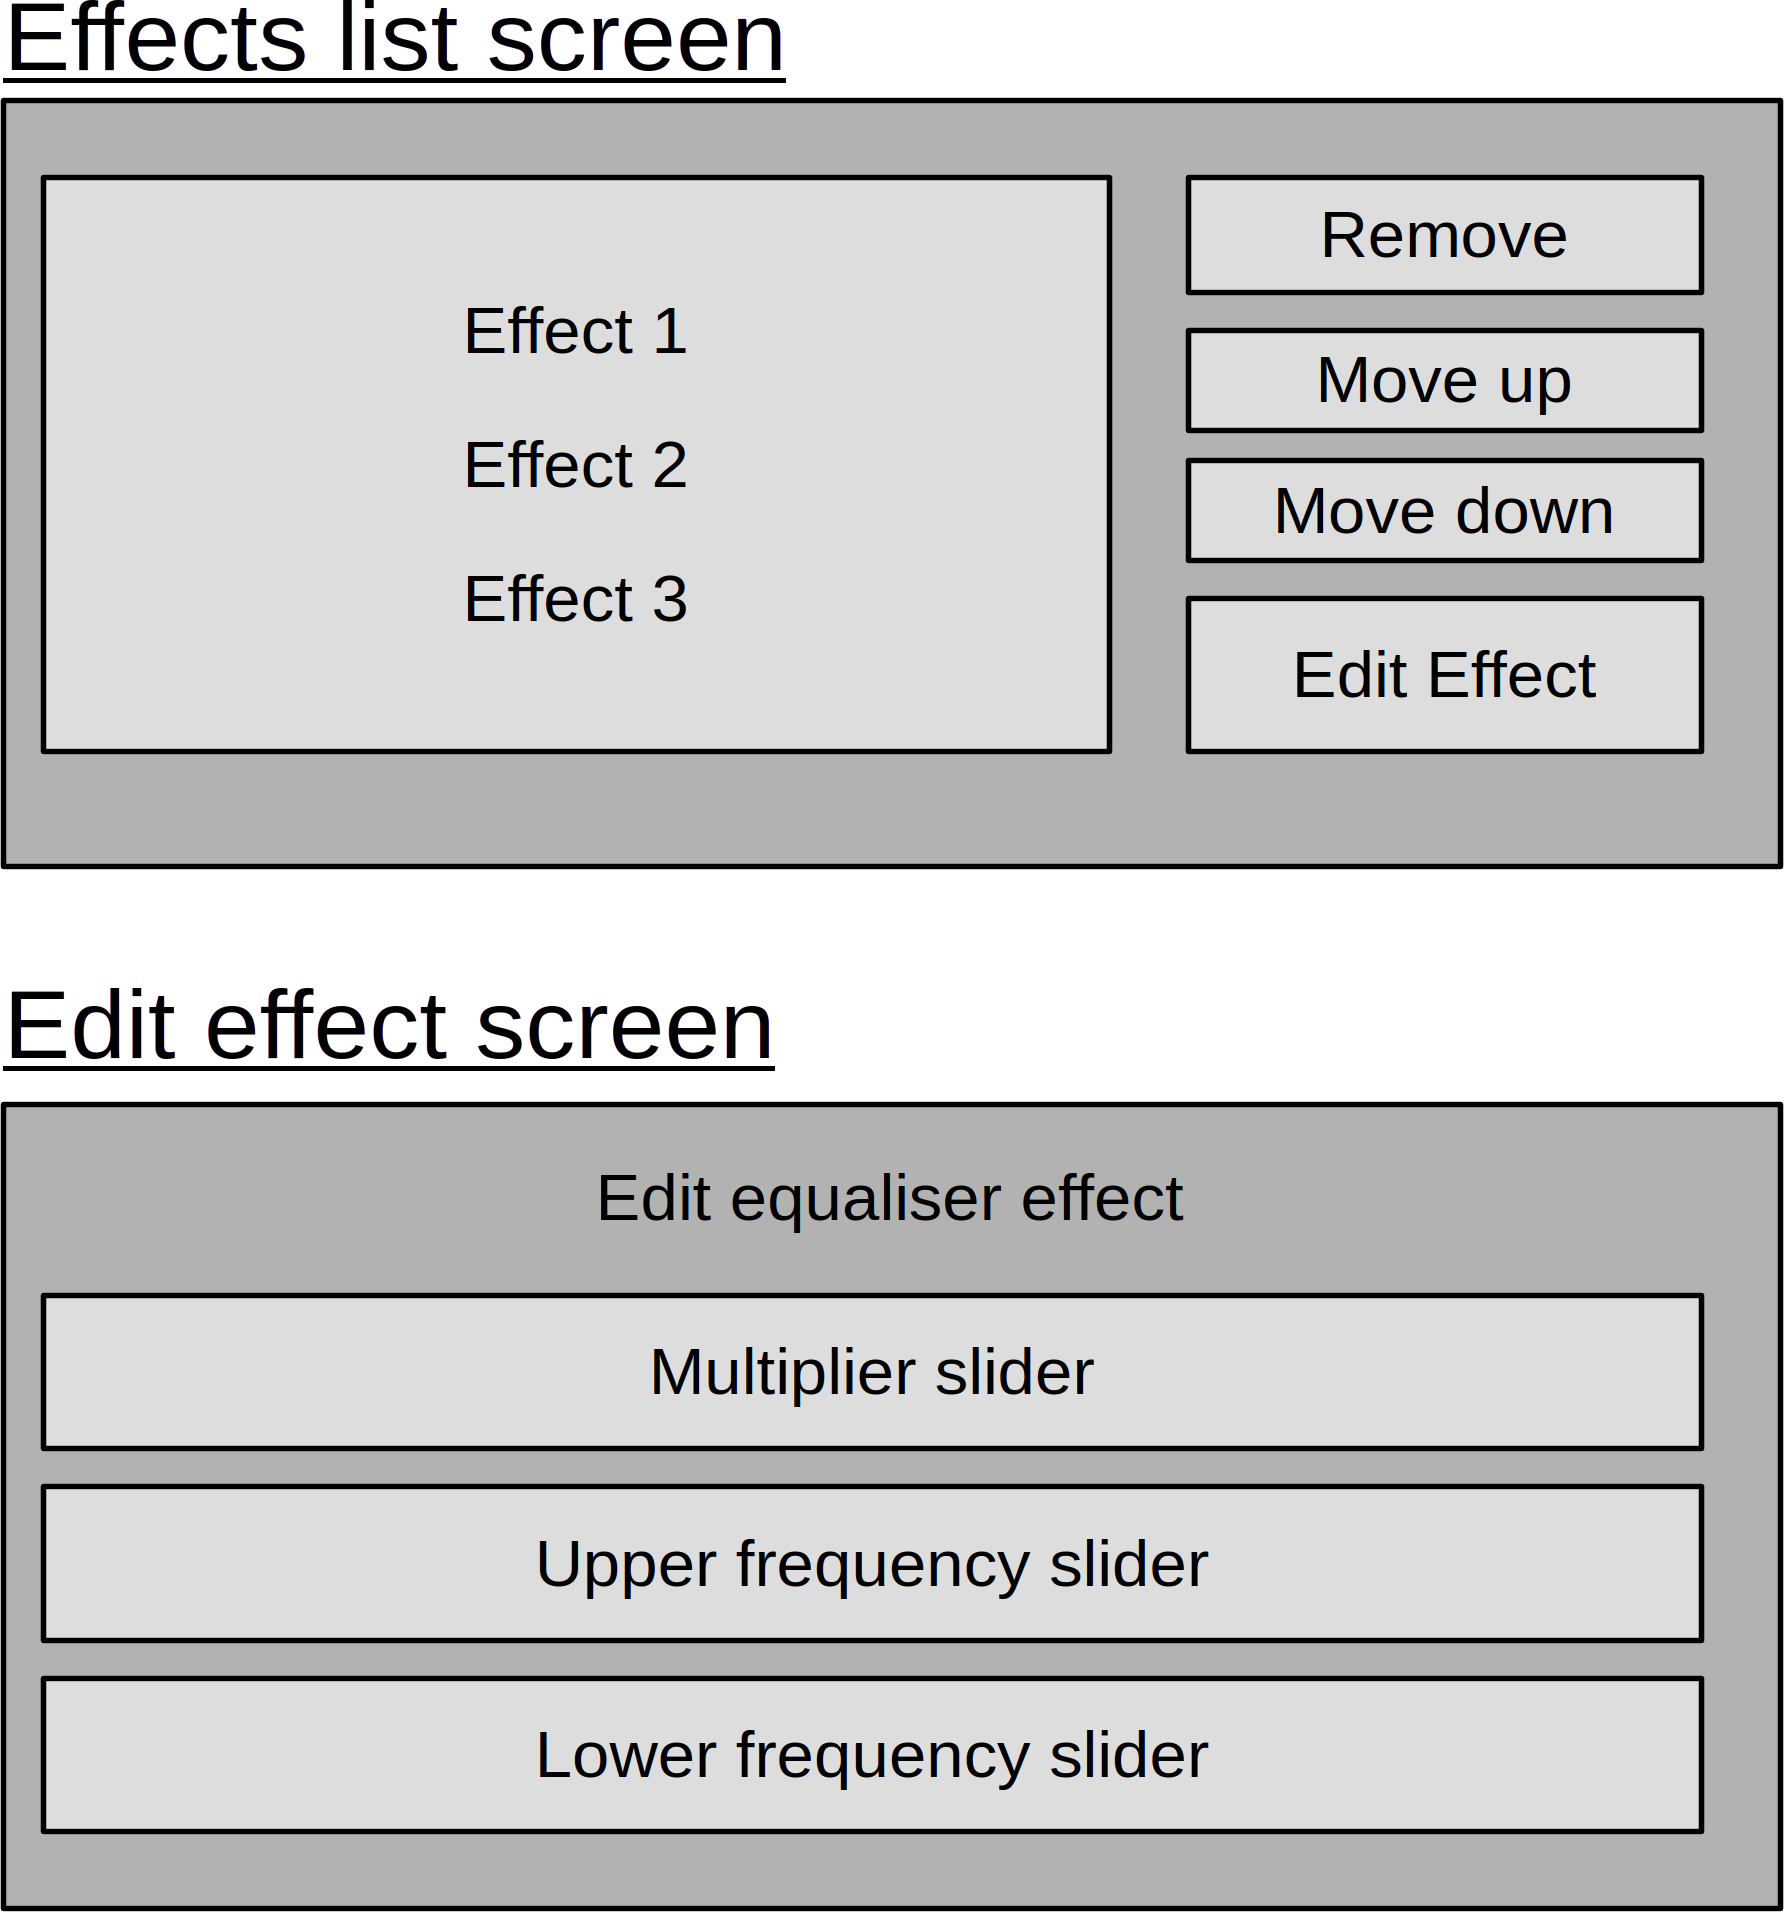
\includegraphics[width=14cm]{./gui wireframes two.png}
	\caption{GUI wireframes for ancillary windows }
\end{figure}

\subsubsection{Relation to the Code}
As I am using "wxWidgets" (see above), all GUIs must be programmed directly in code. I have decided, therefore, to create the following classes to abstract away the details of the GUI:
\begin{itemize}
	\item StartupWindow - implements the initial "choice screen"
	\item PlaylistWindow - implements the "create playlist screen"
	\item FileBrowser - responsible for fetching and drawing the  list of audio files on the system (used by PlaylistWindow). This is abstracted away as "wxWidgets" does not provide a native "widget" for this, so I must create my own.
	\item PlayWindow - implements the "playback screen"
	\item EffectsWindow - implements the "effects list" screen
	\item PropertiesWindow - implements the "edit effect" screen
	\item SongSelectionWindow - draws the popup for when the user chooses to select a new song from the current playlist (abstracted as is non-trivial to implement)
\end{itemize}

\pagebreak
\subsection{Defensive Programming}

\subsubsection{Reading and Writing Audio Files and Playlists}
\paragraph{}
Naturally the program has a need to consume data in various forms. There are three key filesystem operations:
\begin{itemize}
	\item Saving user-created playlists to disk
	\item Loading user-created playlists
	\item Loading audio files from disk
\end{itemize}

\paragraph{}
It should be stressed that any one of these operations could fail. A great many number of edge cases exist:
\begin{itemize}
	\item Upon loading a playlist, one or more audio files referenced may not actually exist
	\item An audio file may be unable to be loaded
	\item The user may lack sufficient permissions to save a playlist to a particular folder (e.g. /root)
	\item The user may input an invalid path when trying to load a playlist
\end{itemize}

\paragraph{}
Thus there is a need to carefully design IO-related subroutines so that, upon the event of failure, the program does not crash or behave incorrectly.

\paragraph{Loading Playlists}
\begin{enumerate}
	\item Upon a playlist file being selected, check it actually exists and can be read
	\item Read the file line by line (where each line corresponds to a path for an audio file)
	\item Verify each audio file actually exists on the system
	\item If an audio file is invalid or cannot be read, further defensive programming (described below when loading audio files themselves) will be employed.
\end{enumerate}

\paragraph{Loading Audio Files}
\begin{enumerate}
	\item When an audio file is loaded by the program (as it's about to be played), raise an exception if, for whatever reason, SDL cannot parse the audio file\footnote{
		Recall that SDL is being used as an audio library to load WAV files. SDL will return an error
		code if it fails, which may occur if the file is corrupt.
	}.
	\item Catch this exception in a try-catch block in the relevant GUI code.
	\item Remove the offending audio file from the playlist \textit{in memory} (not on the filesystem).
	\item If there are other audio files in the playlist, notify the user then skip to them instead (i.e. go to step 1 again).
	\item However if no valid audio files can be found, the entire playlist is invalid. Notify the user then terminate the program.
\end{enumerate}

\paragraph{Saving Playlists}
\begin{enumerate}
	\item Attempt to save the playlist file at the location the user specified.
	\item If the operation returned an error code, inform the user. Due to the control flow of the GUI, there is no need to further alter program flow\footnote{
		This is because the user saves playlists in the "create playlist" window. Once they click save, the window closes, and they are back at the screen presenting them with a choice to load an existing playlist or create a new one, regardless of whether or not the process succeeded. Hence all we need to do is notify the user if something went wrong.
	}.
\end{enumerate}

\subsubsection{Changing Audio Effect Properties}
\paragraph{}
Recall that each audio effect property has a minimum and a maximum value as defined in my UML class diagrams. These will be set explicitly in the code, so that a user cannot, for example, set the "volume property" in the volume effect to a negative number or chose a frequency in the equaliser effect that is outside the range of human hearing.

\paragraph{}
When the relevant GUI sliders are created to allow these properties to be changed, they must have their minimum and maximum values set respectively. This will ensure it is impossible to input invalid settings.

\pagebreak
\subsection{Audio Effect Presets}
\paragraph{}
Presets were idenitifed a key objective in the analysis section, due to the responses received in interviews. The aim is to allow a new user of the software to quickly reach a desired effect, lowering the barrier of entry, whilst also providing an opportunity to showcase how a range of effects can be combined for a particular purpose.

\paragraph{}
I will therefore add a variety of presets to my application, which showcases all of the audio effects at play. To this end I have designed the following presets:
\begin{itemize}
	\item "Far away room" - will apply an echo to make audio sound as if it's coming from a large room, before also applying an equaliser effect to limit higher frequencies\footnote{
		When sound waves are emanated from a source, higher frequencies are typically reflected more frequently (due to their shorter wavelength meaning they "collide" with more objects), and as such attenuate (grow quieter) faster . For example, picture one's self a considerable distance from a party. Typically the bass can still be heard, as well as faint echoes of the vocals, but the higher frequencies have been drowned out as they have lost much more energy reflecting off more objects. Lower frequencies will also typically resonate with the walls of buildings themselves - the exact physics behind this are complex, but thankfully do not need to be understood.
	}.
	\item "Spacious room" - as above, but will instead limit lower frequencies instead\footnote{
		This will make audio sound as if it's being played in a large hall or shopping centre, in which the audio echoes and sounds "tinny" on account of  resonance occurring with the higher frequencies. Again, the precise physics for this do not need to be understood. Rather, this must merely be taken into account.
	}.
	\item "Lo-fi" - Lo-fi refers to a popular genre of remixes in which song are made more "relaxing" by modifying the frequencies present and altering the speed of audio. Sometimes noise is also added.
	\item "Remove bass" - will use the equaliser effect to remove the bass from music.
	\item "Remove treble" - as above, but with treble
	\item "Low-quality speakers" - some people enjoy listening to "lower quality" versions of songs as they find it nostalgic. I will use the equaliser effect to reduce the range of frequencies heard, simulating a low-quality speaker, whilst also adding a small amount of echo and noise to enhance the effect.
\end{itemize}

\paragraph{}
By adding the above effects, many popular "genres" can be accounted for. In addition, all supported audio effects can be showcased to new users in an intuitive way.

\paragraph{}
I have decided to model presets using a functional approach, where each preset is a function, called within the program, that will apply and configure the particular effects required. However, it is unwise to specify, at this point in time, the exact parameters of these presets, as without first having writing the software, one cannot know how for certain how configuration options will behave. Yet broadly speaking, I believe a list of \textit{Preset} structures can be defined, each with a name, speed modifier\footnote{
	The Lo-fi preset will change the speed of audio playback, so I would do well to include this in the preset definition.
} and corresponding function.

\pagebreak
\subsection{Test Design}
\paragraph{}
In order to meet the objectives described in the analysis section, I have decided to design a variety of measurable tests which will indicate if these objectives have been met.
\textbf{For convenience, the objectives from above are repeated below:}

\paragraph{}
{
	\centering
	\fbox{\begin{minipage}{15cm}

			\begin{enumerate}
				\item The user must be able to load a collection of audio files known as a “playlist” and then play the audio
				files contained within, organised alphabetically, as is the custom in audio-listening applications.
				\item  The user must be able to visualise the current audio being played in the frequency domain (i.e. visualise the frequencies)
				\item The user must be able to modify the audio's frequency domain (i.e. selectively modify frequencies such as by reducing the bass)
				\item The user must be able to apply additional "audio effects" to further enhance the music: echo, volume adjustment and noise
				\item The user must be able to configure these "audio effects" individually and also apply pre-made "presets" to quickly reach a desired effect
				\item  The system must run in real-time on an average school computer
				\item The user must be able to alter the speed at which audio is played
			\end{enumerate}

	\end{minipage}}
}

\pagebreak
\subsubsection{Testing Objective 1}
\paragraph{Description} "The user must be able to load a collection of audio files known as a “playlist” and then play the audio
files contained within, organised alphabetically, as is the custom in audio-listening applications."

\paragraph{Test 1.1}
The user must have the option to create a new playlist from a list of audio files on the system.  To test this, I will therefore place a variety of audio files on disk and verify they are detected by the program. Non-audio files will not be able to be selected, for obvious reasons. As the only audio file currently supported is the ".wav" format, any file without this extension will not be displayed.

\paragraph{Test 1.2}
I will then test if playlists created in the program can be successfully saved to disk, then loaded back into the program in a sanitised manner. In other words, playlists consisting solely of files which actually exist on disk should be loaded without error (such that audio playback starts), but playlists with non-existent audio files should fail to load and notify the user of the error.

\paragraph{Test 1.3}
After loading a playlist and beginning audio playback, the audio files contained within must appear alphabetically in the audio file selection screen, ordered in ascending order by their respective filenames.

\paragraph{Test 1.4}
Any invalid audio files should be skipped over, and should not crash the program. The user should be notified if this happens.

\paragraph{Test 1.5}
The playlist's shuffle subroutine is able to correctly randomise the order of audio files.

\paragraph{Test 1.6}
Audio playback (without any effects applied, on valid files) works correctly.

\paragraph{Test 1.7}
The program is able to correctly determine the key properties of audio files (frequency and number of channels).

\paragraph{}

\pagebreak
\subsubsection{Testing Objective 2}
\paragraph{Description} "The user must be able to visualise the current audio being played in the frequency domain (i.e. visualise the frequencies)"

\paragraph{}
As it is difficult for humans to visualise the frequency domain of audio themselves, I will generate audio files consisting of a sine wave of a constant, known frequency. Thus, when the frequency domain is visualised, there should be a single visual peak corresponding to the chosen frequency. By testing the visualisation in this manner across a range of frequencies, it should therefore be possible to deduce if the visualisation is correct.

\paragraph{}
Obviously the vast majority of audio being played will consist of multiple frequencies. I will therefore combine multiple sine waves in a single audio file (e.g. 500 Hz and 1000 Hz, both playing at the same time). Thus there should be multiple identifiable peaks, each one corresponding to a sine wave frequency chosen.

\paragraph{}
It should be stressed that human hearing only extends from 20 Hz to 20,000 Hz, and as such any audio visualisation must exclude frequencies outside these ranges.

\paragraph{}
In addition to testing the visualisation output itself, I will  also test that the corresponding subroutines that it depends on are also functioning correctly. For example, the visualisation maths depends on being able to convert between real and complex (as in complex numbers) representations of audio. It also depends on correctly using the Bark scale.

\begin{figure}[H]
	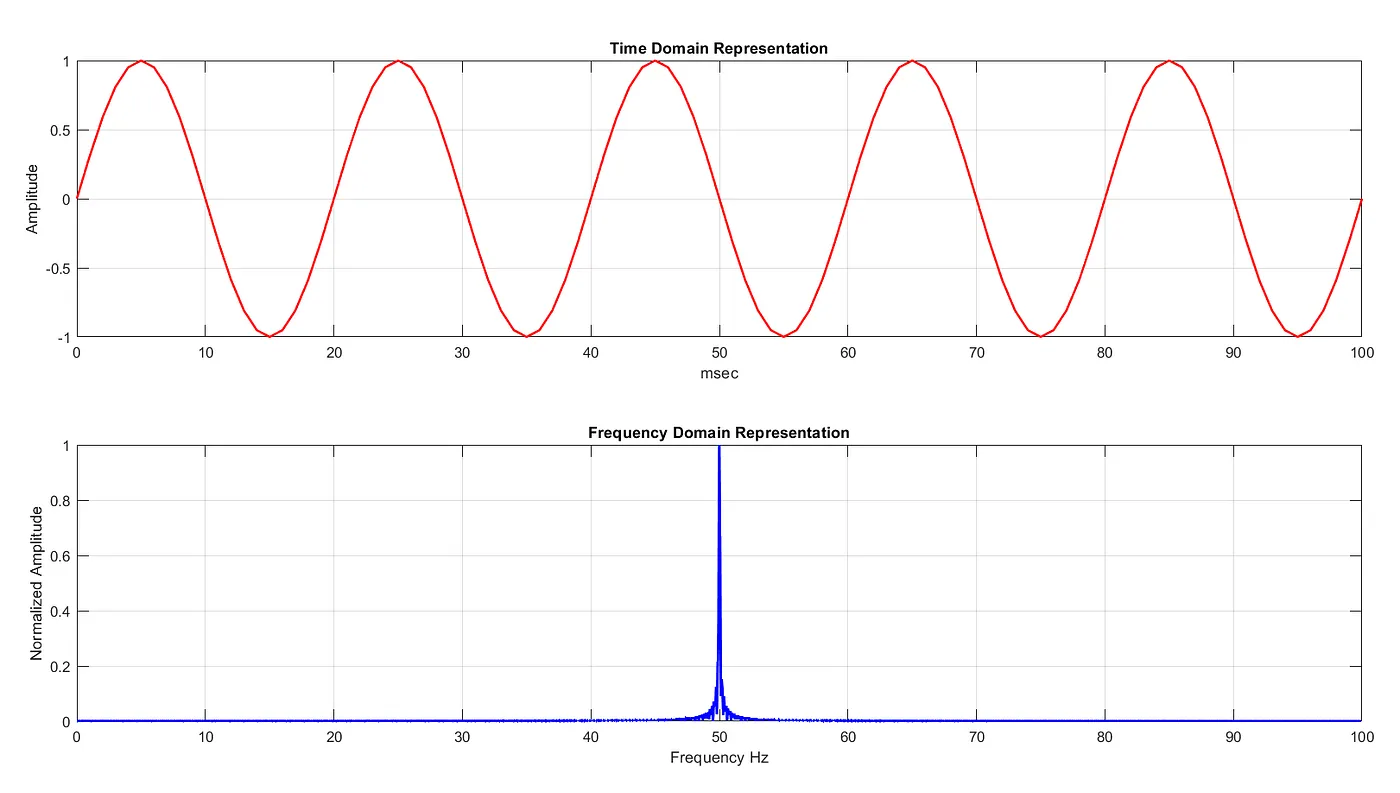
\includegraphics[width=14cm]{./fft test example.png}
	\caption{An example piece of audio, with the time domain shown above and the frequency domain below. If my tests succeed, they should look similar to the first picture (multiple sine waves will of course have multiple peaks of this nature). }
	% Credit - Aniket Kamat: https://aniket-kamat.medium.com/demystifying-the-fourier-transform-a995bdb6d73a
\end{figure}

\paragraph{Test 2.1} A correct visualisation of a sine wave is apparent at 500 Hz, with a single peak corresponding to that frequency.
\paragraph{Test 2.2} A correct visualisation of a sine wave is apparent at 1,000 Hz, with a single peak corresponding to that frequency.
\paragraph{Test 2.3} Sine waves outside the human audible range, at 10 Hz and 30,000 Hz respectively, produce no visible output, as they are inaudible.
\paragraph{Test 2.4} A correct visualisation of two sine waves (one at 1,000 Hz and one at 10,000 Hz) is apparent, with two separate peaks corresponding to those frequencies.
\paragraph{Test 2.5} A correct visualisation of three sine waves (1,000 Hz, 5,000 Hz and 15,000 Hz ) is apparent, with three separate peaks corresponding to those frequencies.
\paragraph{Test 2.6} Audio samples are correctly converted to complex form
\paragraph{Test 2.7} When assessing loudness, a correct conversion from the Hertz to the Bark Scale occurs

\pagebreak
\subsubsection{Testing Objective 3}
\paragraph{Description} "The user must be able to modify the audio's frequency domain (i.e. selectively modify frequencies such as by reducing the bass)"

\paragraph{Test 3.1}
The program's equaliser effect is able to selectively reduce the bass of any given audio (corresponding to the low frequencies in frequency space).

\paragraph{Test 3.2}
The program's equaliser effect is able to selectively reduce the treble of any given audio (corresponding to the high frequencies in frequency space).

\paragraph{Test 3.3}
The program's equaliser effect is able to correctly reduce the magnitude of complex audio samples in frequency space without affecting their phase.

\paragraph{}
A more general test, involving a variety of frequencies and amplitudes, is also wished to be conducted. However, such a test has already been designed - see test 5.3. Thus objective 3 can also be considered to be tested via this test, which for the convenience of the reader is repeated below:

\paragraph{Test 5.3} "The equaliser effect can have its various parameters modified, which results in a correct change in the audio playback, such that any required range of frequencies can have its amplitude modified in any way."

\paragraph{Verifying Results}
I will verify the results both by ear and using the audio visualiser\footnote{
	For example, if one chooses to reduce the bass, then the parts
	of the visualisation corresponding to the lower frequencies must
	visually appear smaller in relation to the other frequencies.
}, so as the ensure that the program is able to selectively reduce the range of frequencies chosen.

\pagebreak
\subsubsection{Testing Objective 4 (including use of subject specialist)}
\paragraph{Description} "The user must be able to apply additional "audio effects" to further enhance the music: echo, volume adjustment and noise"

\paragraph{}
Due to the subjective nature of audio effects, I will ask multiple people from the program's target audience to provide in-depth feedback on all the audio effects.

\paragraph{}
Recall that the goal of this project is to assist in the user-friendly and convenient creation of song remixes, and so I will ask them to verify that the audio effects produced by the program mimic the effects typically heard in said remixes.

\paragraph{}
At least one of these people will be someone experienced in audio processing, so that they are able to assess if the effects provided sound physically accurate
(particularly the echo). I plan on using my Maths teacher Mr Godwin for this (referred to in later sections as the "Subject Specialist"), as he has experience in Digital Signal Processing (particularly as it relates to audio) from his university degree in Maths, and has a keen ear for audio. He also has experience in sound production at live events, so will be knowledgeable about what a correct echo will sound like.

\paragraph{Test 4.1} A select group from the target audience certify that the echo effect sounds physically plausible, and mimics the effect as it is commonly heard in song remixes
\paragraph{Test 4.2} A select group from the target audience certify  that the noise effect sounds physically plausible, and mimics the effect as it is commonly heard in song remixes
\paragraph{Test 4.3} The volume effect can be seen to adjust the volume correctly

\pagebreak
\subsubsection{Testing Objective 5}
\paragraph{Description} "The user must be able to configure these "audio effects" individually, yet also apply pre-made "presets" to quickly reach a desired effect"

\paragraph{Test 5.1} The noise effect can have its various parameters modified, which results in a correct change in the audio playback.
\paragraph{Test 5.2} The echo effect can have its various parameters modified, which results in a correct change in the audio playback.
\paragraph{Test 5.3} The equaliser effect can have its various parameters modified, which results in a correct change in the audio playback, such that any required range of frequencies can have its amplitude modified in any way.
\paragraph{Test 5.4} All presets present in the application can be loaded successfully, with the appropriate audio effects having been added and configured correctly, such that the desired effect is reached.

\paragraph{}
There is no need to test the volume effect here, as configuring it was already covered in test 4.3.

\pagebreak
\subsubsection{Testing Objective 6}
\paragraph{Description}  "The system must run in real-time on an average school computer"

\paragraph{}
I will test the performance of the program by running it on a computer in my school, which represents more-or-less average school hardware.
I will also test it on my school laptop too, which has more modest hardware, to ensure that in all contexts in which a student might run the program, there will be no performance issues. If possible, I may also attempt to test the software on even less powerful hardware (such as a decade-old laptop) to highlight room for potential growth.
In order to appear to run in real-time\footnote{
As per the definition of "real-time" used within this document - see the preface}
, there must be no noticeable delay in the audio or the visuals, such that the following must be observed:
\begin{enumerate}
	\item Audio should be processed in under 3 milliseconds\footnote{
		This is widely considered the minimum delay that can be perceived by the human brain, though estimates vary from 3ms to as much as 30 -  see https://legacy.presonus.com/learn/technical-articles/Digital-Audio-Latency-Explained and https://www.churchproduction.com/education/latency-and-its-affect-on-performers/
	}
	\item The visualisation graphics must update in less than 16.6 ms, such that it is displayed at 60 frames per second, which is the most common refresh rate on school hardware. This will be measured by the code itself as it's running.\footnote{
		This is considered the "benchmark" for most real-time systems (in the sense of the word employed in the preface - see the top of the document). As long as the program outputs visuals at least as fast as the monitor displays them,  there will be no noticeable "lag" or delay.
	}
\end{enumerate}

\paragraph{}
To actually time the code, the following pseudo-code will be temporarily added to the relevant subroutines:
\begin{minted}{ada}
function process_audio:
	start_time := measure_time()
	-- rest of code here
	end_time := measure_time()
	duration := end_time - start_time()
	time_in_ms := to_milliseconds(duration)
	print("audio took " + time_in_ms + " ms")

function process_visuals:
	start_time := measure_time()
	-- rest of code here
	end_time := measure_time()
	duration := end_time - start_time()
	time_in_ms := to_milliseconds(duration)
	print("visuals took " + time_in_ms + " ms")
\end{minted}

\paragraph{Test 6.1} The program must run, without any effects applied, in real-time on the specified hardware.
\paragraph{Test 6.2} The program must run in real-time, with every effect applied at once, in real-time on the specified hardware.

\pagebreak
\subsubsection{Testing Objective 7}
\paragraph{Description} "The user must be able to alter the speed at which audio is played"

\paragraph{Test 7.1} The program must be able to play  back audio at an increased speed
\paragraph{Test 7.2} The program must be able to play back audio at a reduced speed
\paragraph{Test 7.3} Speeding up audio playback does not significantly increase the computational overhead (to fulfil objective 6)
\paragraph{Test 7.4} Slowing down audio playback does not significantly increase the computational overhead (to fulfil objective 6)

\pagebreak
\subsection{Final overview of project hierarchy}
\begin{figure}[H]
	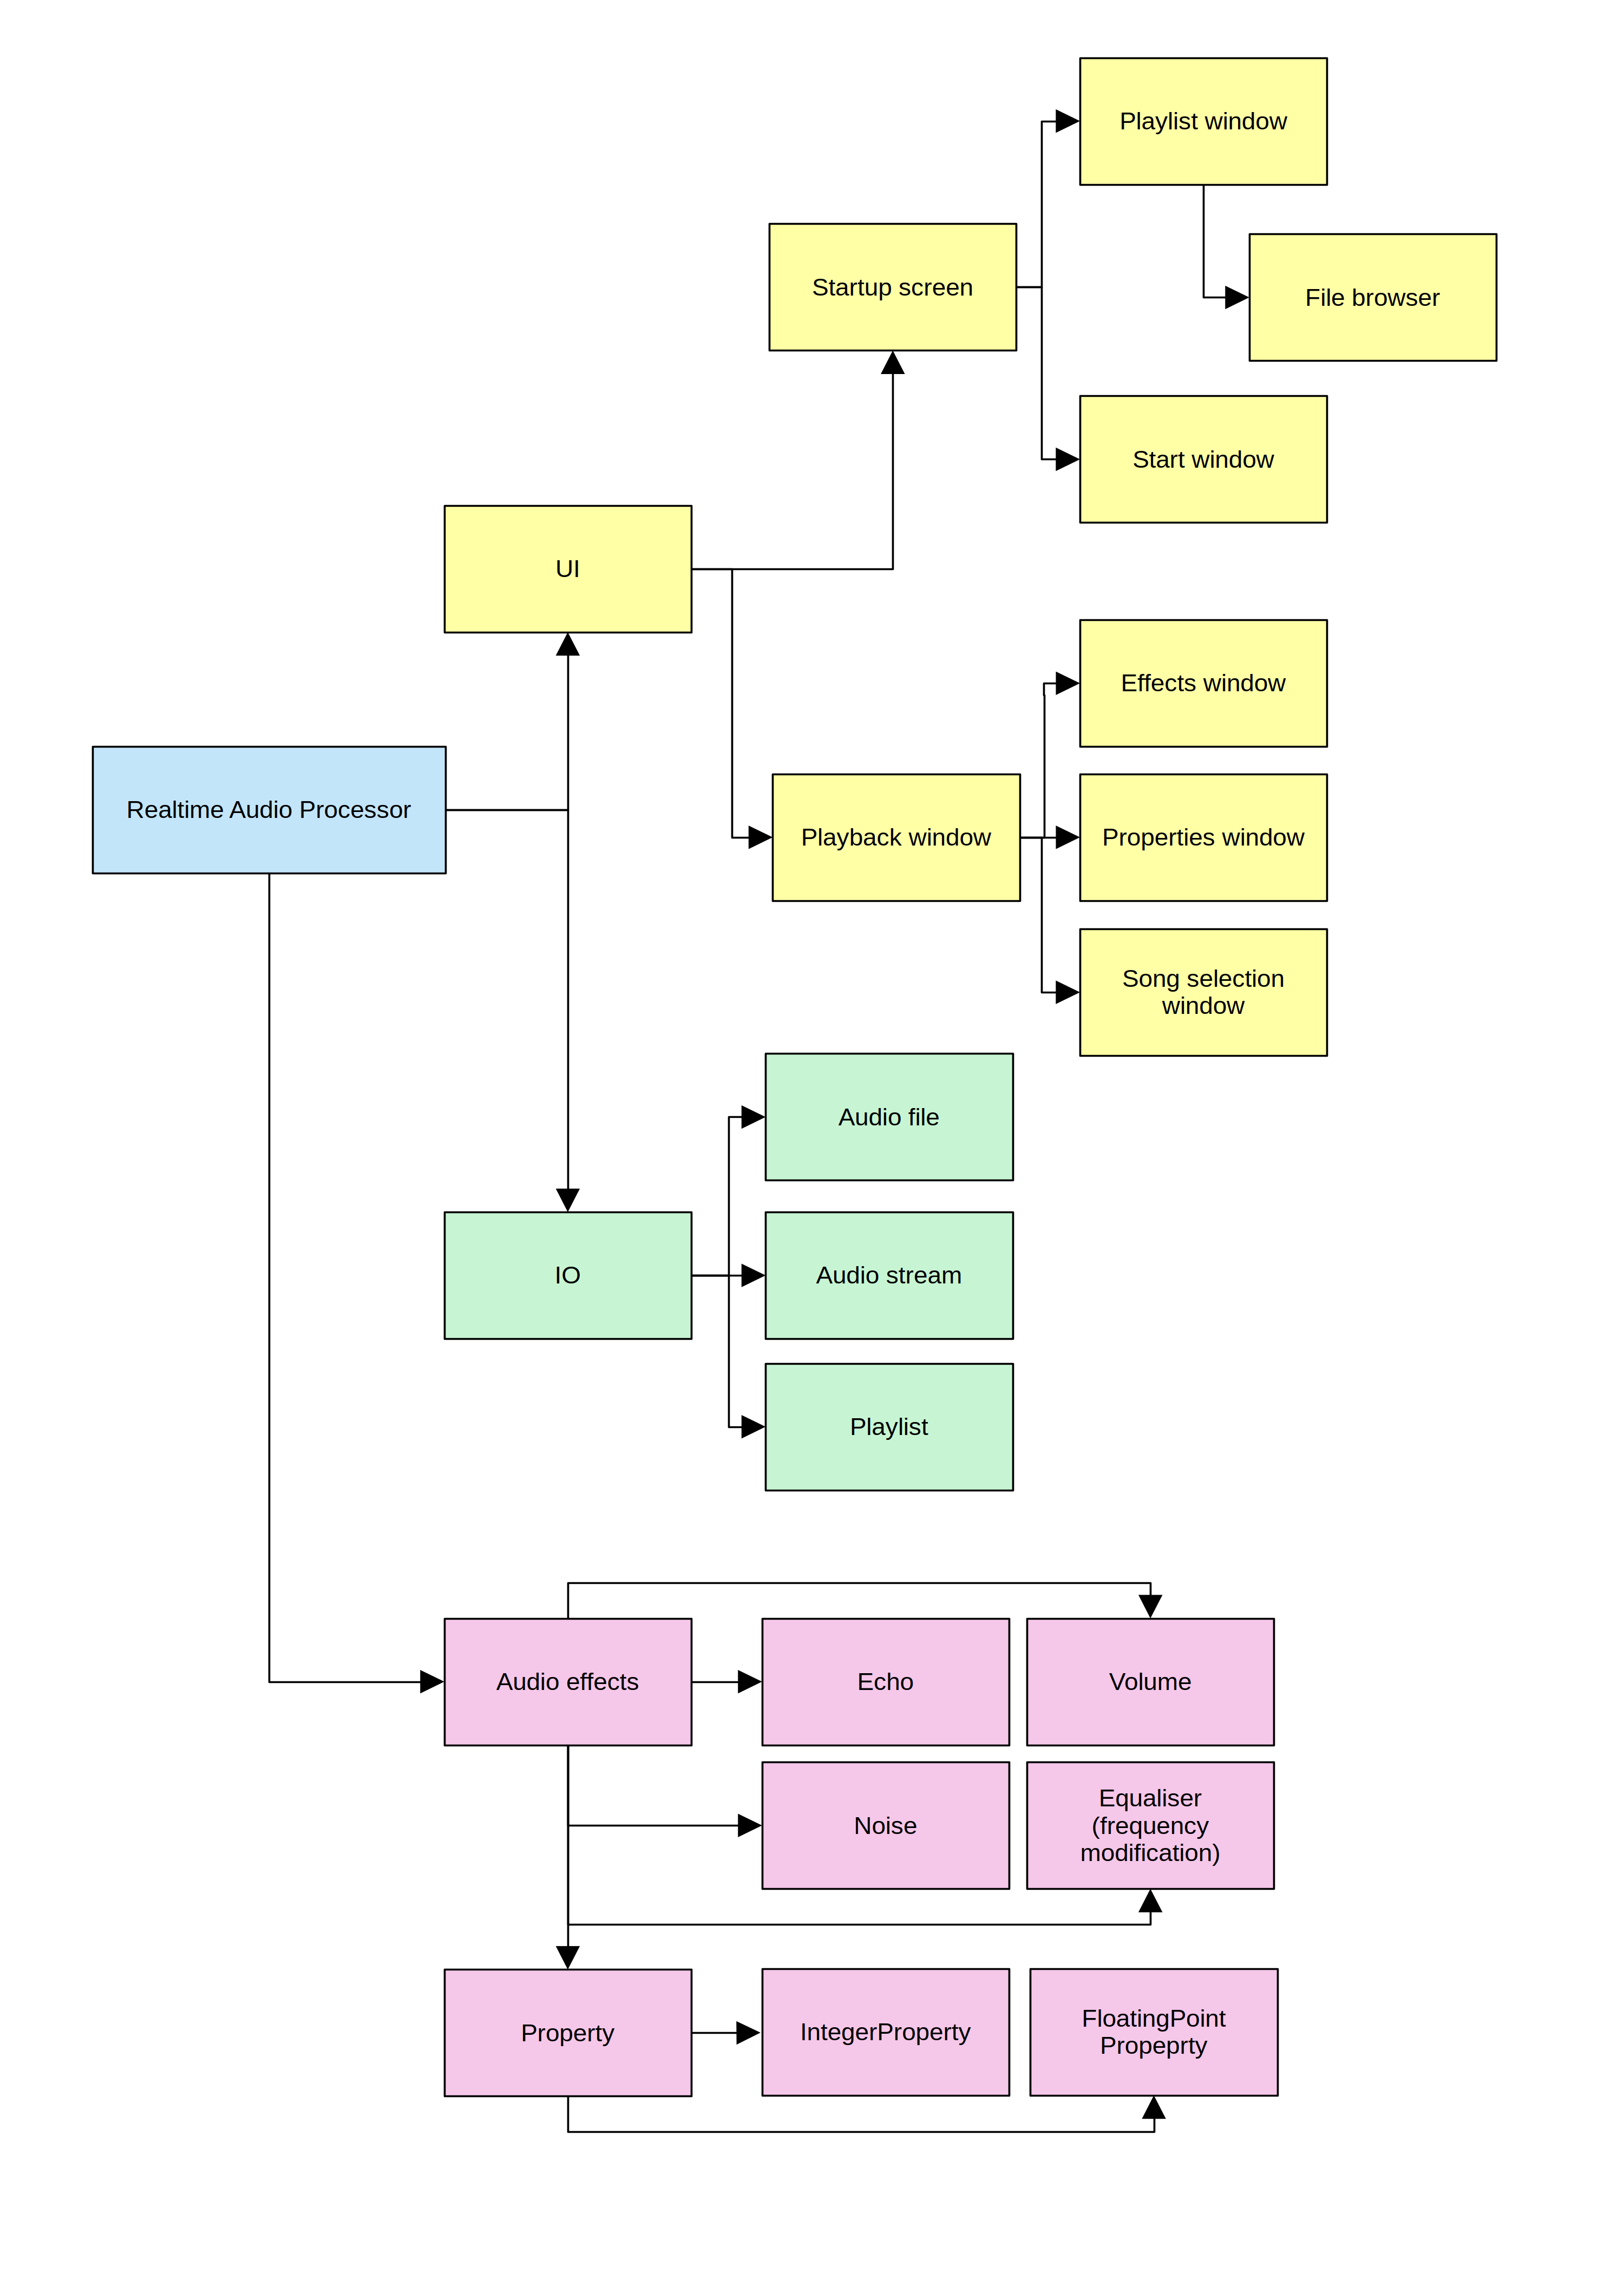
\includegraphics[width=14cm]{./hierarchy chart.png}
	\caption{Hierarchy chart}
\end{figure}
